\documentclass[10pt]{article}

\title{Program Assigment - RNA Secondary Structure Prediction}
\date{\today}
\author{Weize Xu}


\usepackage{geometry}
\geometry{
    a4paper,
    total={170mm,257mm},
    left=30mm,
    right=20mm,
    top=20mm,
    }
\usepackage{listings}
\lstset{basicstyle=\ttfamily\footnotesize,breaklines=true}
\usepackage{amsmath}
\usepackage{hyperref}
\usepackage{makecell}
\usepackage{graphicx}
\usepackage{subcaption}


\begin{document}

\maketitle

\section{About the Program}

\subsection{Dependency}
This program is develop and tested under Linux system,
and Python version $\geq$ 3.4 is required.

\subsection{Usage}

Open your shell, and type "python main.py --help" to show the usage information, as follow:

\begin{lstlisting}[frame=single]
$ python main.py --help
usage: RNA-2nd-structure-predictor [-h]
                                   [--method [{nussinov,maxstacks,minstackenergy}]]
                                   [--print_max_score]
                                   input

Predict the secondary structure of an RNA sequence.

positional arguments:
  input                 Path to input fasta file.

optional arguments:
  -h, --help            show this help message and exit
  --method [{nussinov,maxstacks,minstackenergy}]
                        Algorithm used for predict.
  --print_max_score, -v
                        Print the max score.
\end{lstlisting}

\section{Algorithms for each Task}

\subsection{Maximize the number of base pairs}
Just use the Nussinov algorithm.

\subsubsection{Implementation}

See Python module \url{./nussinov.py}

\subsection{Maximize the number of stacking pairs}
\label{sec:max_stack}
Solving with a dynamic programming,
it's very like the Nussinov algorithm, just a little different:

\subsubsection{Algorithm description}
\noindent
\textbf{Notation:}

\begin{center}
    \begin{tabular}{{l} {l}}
        $S[1..n]$ & An RNA sequence with $n$ bases. \\
        $V(i, j)$ & The maxmium number of stacking pairs in $S[i,j]$\\
    \end{tabular}
\end{center}

\noindent
\textbf{Basic case:}

\begin{center}
    $V(i,j) = 0$ \textbf{if} $j < j+3$
\end{center}

Since, when $j < i + 3$, it can not form a stacked pair.
The shortest span length stacking pair looks like this:

\begin{lstlisting}[xleftmargin=.4\textwidth]
    i  j
....AAUU....
    (())
\end{lstlisting}

\noindent
\textbf{Recursive case:}

\begin{enumerate}  
    \item No stacked pair in position j:
    \begin{center} $V(i,j)=V(i,j-1)$ \end{center}
    \item No stacked pair in position i:
    \begin{center} $V(i,j)=V(i+1,j)$ \end{center}
    \item Position $(i,j)$ form a length $h$ stacking pairs:
    \begin{equation}
    \label{eq:max_stack_case3}
    V(i,j)=\max_{1 \leq h \leq m }{
        \{ V(i+h+1,j-h-1)+ h* \prod_{t=0}^{h} \delta(S[i+t], S[j-t]) \}
    }
    \end{equation}
    Where:
    \begin{center} $m = floor(\dfrac{i-j+1}{2})-1$ \end{center}
    \begin{center} $\delta(x,y)=1$ \textbf{if} $(x,y) \in P$ \textbf{otherwise} $0$ \end{center}
    \begin{center} $P = \{(a,u),(u,a),(c,g),(g,c),(g,u),(u,g)\}$ \end{center}
    \item Both position $i$ and $j$ form a stacking pair, but $(i,j)$ not form stacking pair:
    \begin{center} $V(i,j) = \displaystyle\max_{i+3\leq k<j}\{V(i,k) + V(k+1,j)\}$ \end{center}
\end{enumerate}

So, the recursive function is:
\begin{equation}
    V(i,j)=\max\begin{cases}
        V(i,j-1) \\
        V(i+1,j) \\
        \displaystyle\max_{1 \leq h \leq m }{ \{ V(i+h+1,j-h-1)+ h* \prod_{t=0}^{h} \delta(S[i+t], S[j-t]) \}} \\
        \displaystyle\max_{i+3\leq k<j}\{V(i,k) + V(k+1,j)\}
    \end{cases}
\end{equation}

\noindent
\subsubsection{Complexity Analyze}
\label{ana:max_stack}

Space used for store the $V(i, j)$ is $O(n^2)$.
Time needed to fill the $V(i, j)$ entries is $O(n^2)$,
and each $V(i,j)$ entry can be computed in $O(n)$ time.
So this algorithm can be solved in $O(n^3)$ time.
This complexity is same to the Nussinov algorithm.

\subsubsection{Implementation}

See Python module \url{./maxstacks.py}

\subsection{Minimize free energy of stacking pairs}

\subsubsection{Algorithm description}

This method is a simpler version of minimum free energy method(MSE),
only consider the free energy of stacking pairs.
The free energy of stacking pair $eS$ is get from the Turner table: 

\begin{center}
    \begin{tabular}{|{l}|{c}|{c}|{c}|{c}|{c}|{c}|}
        \hline
         & A/U & C/G & G/C & U/A & G/U & U/G \\ \hline
        A/U & $-0.9$ & $-2.2$ & $-2.1$ & $-1.1$ & $-0.6$ & $-1.4$ \\ \hline
        C/G & $-2.1$ & $-3.3$ & $-2.4$ & $-2.1$ & $-1.4$ & $-2.1$ \\ \hline
        G/C & $-2.4$ & $-3.4$ & $-3.3$ & $-2.2$ & $-1.5$ & $-2.5$ \\ \hline
        U/A & $-1.3$ & $-2.4$ & $-2.1$ & $-0.9$ & $-1.0$ & $-1.3$ \\ \hline
        G/U & $-1.3$ & $-2.5$ & $-2.1$ & $-1.4$ & $-0.5$ & $+1.3$ \\ \hline
        U/G & $-1.0$ & $-1.5$ & $-1.4$ & $-0.6$ & $+0.3$ & $-0.5$ \\ \hline
    \end{tabular}
\end{center}

Actually, we just need to make a small modify to the algorithm in the section \ref{sec:max_stack}.
We can just change the equation \ref{eq:max_stack_case3} in recursive case 3 to:

\begin{equation}
    \label{eq:mspe_case3}
    V(i,j) =\max_{1\leq h \leq m}{\{ V(i+h+1,j-h-1) - \sum_{t=0}^{h} eS(i+t, j-t) * \prod_{t=0}^{h} \delta(S[i+t], S[j-t]) \}}
\end{equation}

Where the $eS(i,j)$ can get from the RNA sequence and the Turner table.
Here we maxmized the negative free energy of stacking pairs, it equal to
minimize it. \\

\noindent
\textbf{Penalty for short distance pairs:}\\

Actually, this algorithm is not good enough.
We can penalize the short distance pairs for get a more closer result,
because the short distance pairs have larger energy in general.
Here we define a penalty function $P(i,j)$:

\[
    P(i,j) = \dfrac{1}{1+a^{-b((i-j)-c)}}
\]

$a$, $b$ and $c$ are positive constants. Then, put it into the recursive function \ref{eq:mspe_case3}:

\[
    V(i,j) =\max_{1\leq h \leq m}{\{ V(i+h+1,j-h-1) - \sum_{t=0}^{h} P(i+t,j-t)eS(i+t, j-t) * \prod_{t=0}^{h} \delta(S[i+t], S[j-t]) \}}
\]


\subsubsection{Complexity Analyze}

Same to section \ref{ana:max_stack}.

\subsubsection{Implementation}

See Python module \url{./minstackenergy.py} \\

\noindent
The advantage and disadvantage about this method is disscused in section \ref{discussion}.

\section{Benchmark on Testing Data}
\subsection{Run algorithms on the testing data}

Firstly run the Nussinov algorithm:
\begin{lstlisting}[frame=single,breaklines=false]
$ python main.py test_data/hammerhead_ribozyme.fa --print_max_score --method nussinov
> hammerhead ribozyme (1rmn)
GCGCUCUGAUGAGGCCGCAAGGCCGAAACUGCCGCAAGGCAGUCAGCGC
((()((((()(.(()(()(.(()()...))))).)).)())))(.()).
20
$ python main.py test_data/PDB_00313.fa --print_max_score --method nussinov
> PDB_00313 (E. Coli) CYSTEINYL-TRNA
GGCGCGUUAACAAAGCGGUUAUGUAGCGGAUUGCAAAUCCGUCUAGUCCGGUUCGACUCCGGAACGCGCCUCCA
(((())(()))(..(((()(()((((((((((()))()(.))(())))())))()))((())))()))).))..
34
$ python main.py test_data/SRP_00004.fa  --print_max_score --method nussinov
> SRP_00004
GGGAGGUUGGUGGUGGACGAGCCACUCGCCAACCGGGUCAGGUCCGGAAGGAAGCAGCCCUAACGAGCCAGGCACGGGUCGCCGUGCC
AGCCUCCCACCUUUU
(((((()(((((()((.().())(.)())))((())(((.)(((())).((..((.)))(().().))))(((((((()()))))))(
.)))))).)).))))
45
\end{lstlisting}

\noindent
As shown above the max score(maximum pairs) get from the Nussinov algorithm is 20, 34 and 45.\\

\pagebreak

\noindent
Then the maximum stacking pairs method:

\begin{lstlisting}[frame=single,breaklines=false]
$ python main.py test_data/hammerhead_ribozyme.fa --print_max_score --method maxstacks
> hammerhead ribozyme (1rmn)
GCGCUCUGAUGAGGCCGCAAGGCCGAAACUGCCGCAAGGCAGUCAGCGC
((((((.))(((((((....))))....(((((....))))))))))))
13
$ python main.py test_data/PDB_00313.fa --print_max_score --method maxstacks
> PDB_00313 (E. Coli) CYSTEINYL-TRNA
GGCGCGUUAACAAAGCGGUUAUGUAGCGGAUUGCAAAUCCGUCUAGUCCGGUUCGACUCCGGAACGCGCCUCCA
((((((((.(((.(((.))).))).(((((((...)))))))..((((.(()).))))(())))))))))....
22
$ python main.py test_data/SRP_00004.fa  --print_max_score --method maxstacks
> SRP_00004
GGGAGGUUGGUGGUGGACGAGCCACUCGCCAACCGGGUCAGGUCCGGAAGGAAGCAGCCCUAACGAGCCAGGCACGGGUCGCCGUGCC
AGCCUCCCACCUUUU
(((((((.((((((((.....)))((((((.(((.)))..))((()))(((..((.)))))..)))))))(((((((....)))))))
((.)))).)))))))
29
\end{lstlisting}

\noindent
The max stacking pairs of three samples are 13, 22 and 29.\\

\noindent
Then run the minimize stacking pairs energy method.

\begin{lstlisting}[frame=single,breaklines=false]
$ python main.py test_data/hammerhead_ribozyme.fa --print_max_score --method
minstackenergy
> hammerhead ribozyme (1rmn)
GCGCUCUGAUGAGGCCGCAAGGCCGAAACUGCCGCAAGGCAGUCAGCGC
((((((....))((((....))))((..(((((....))))))).))))
34.47232640482083
$ python main.py test_data/PDB_00313.fa --print_max_score --method minstackenergy
> PDB_00313 (E. Coli) CYSTEINYL-TRNA
GGCGCGUUAACAAAGCGGUUAUGUAGCGGAUUGCAAAUCCGUCUAGUCCGGUUCGACUCCGGAACGCGCCUCCA
((((((((((((((....)).))).(((((((...))))))).)).(((((.(())..))))))))))))....
47.1048578347625
$ python main.py test_data/SRP_00004.fa  --print_max_score --method minstackenergy
> SRP_00004
GGGAGGUUGGUGGUGGACGAGCCACUCGCCAACCGGGUCAGGUCCGGAAGGAAGCAGCCCUAACGAGCCAGGCACGGGUCGCCGUGCC
AGCCUCCCACCUUUU
(((.((((((.(((((.....)))))..))))))(((((((((((....))).((.)))))...))((..(((((((....)))))))
.))..))).)))...
66.78663059444345
\end{lstlisting}

\subsection{Compare with correct structure}
\label{sec:compare}
Then we can compare the results from each algorithms with the correct structure by visualize them.
I have visualized them with forna(\url{http://rna.tbi.univie.ac.at/forna/}),
results is shown in the Fig.\ref{fig:harmmerhead}, \ref{fig:PDB_00313} and \ref{fig:SRP_00004}.

\begin{figure}[p]
    \begin{subfigure}[b]{0.2\linewidth}
        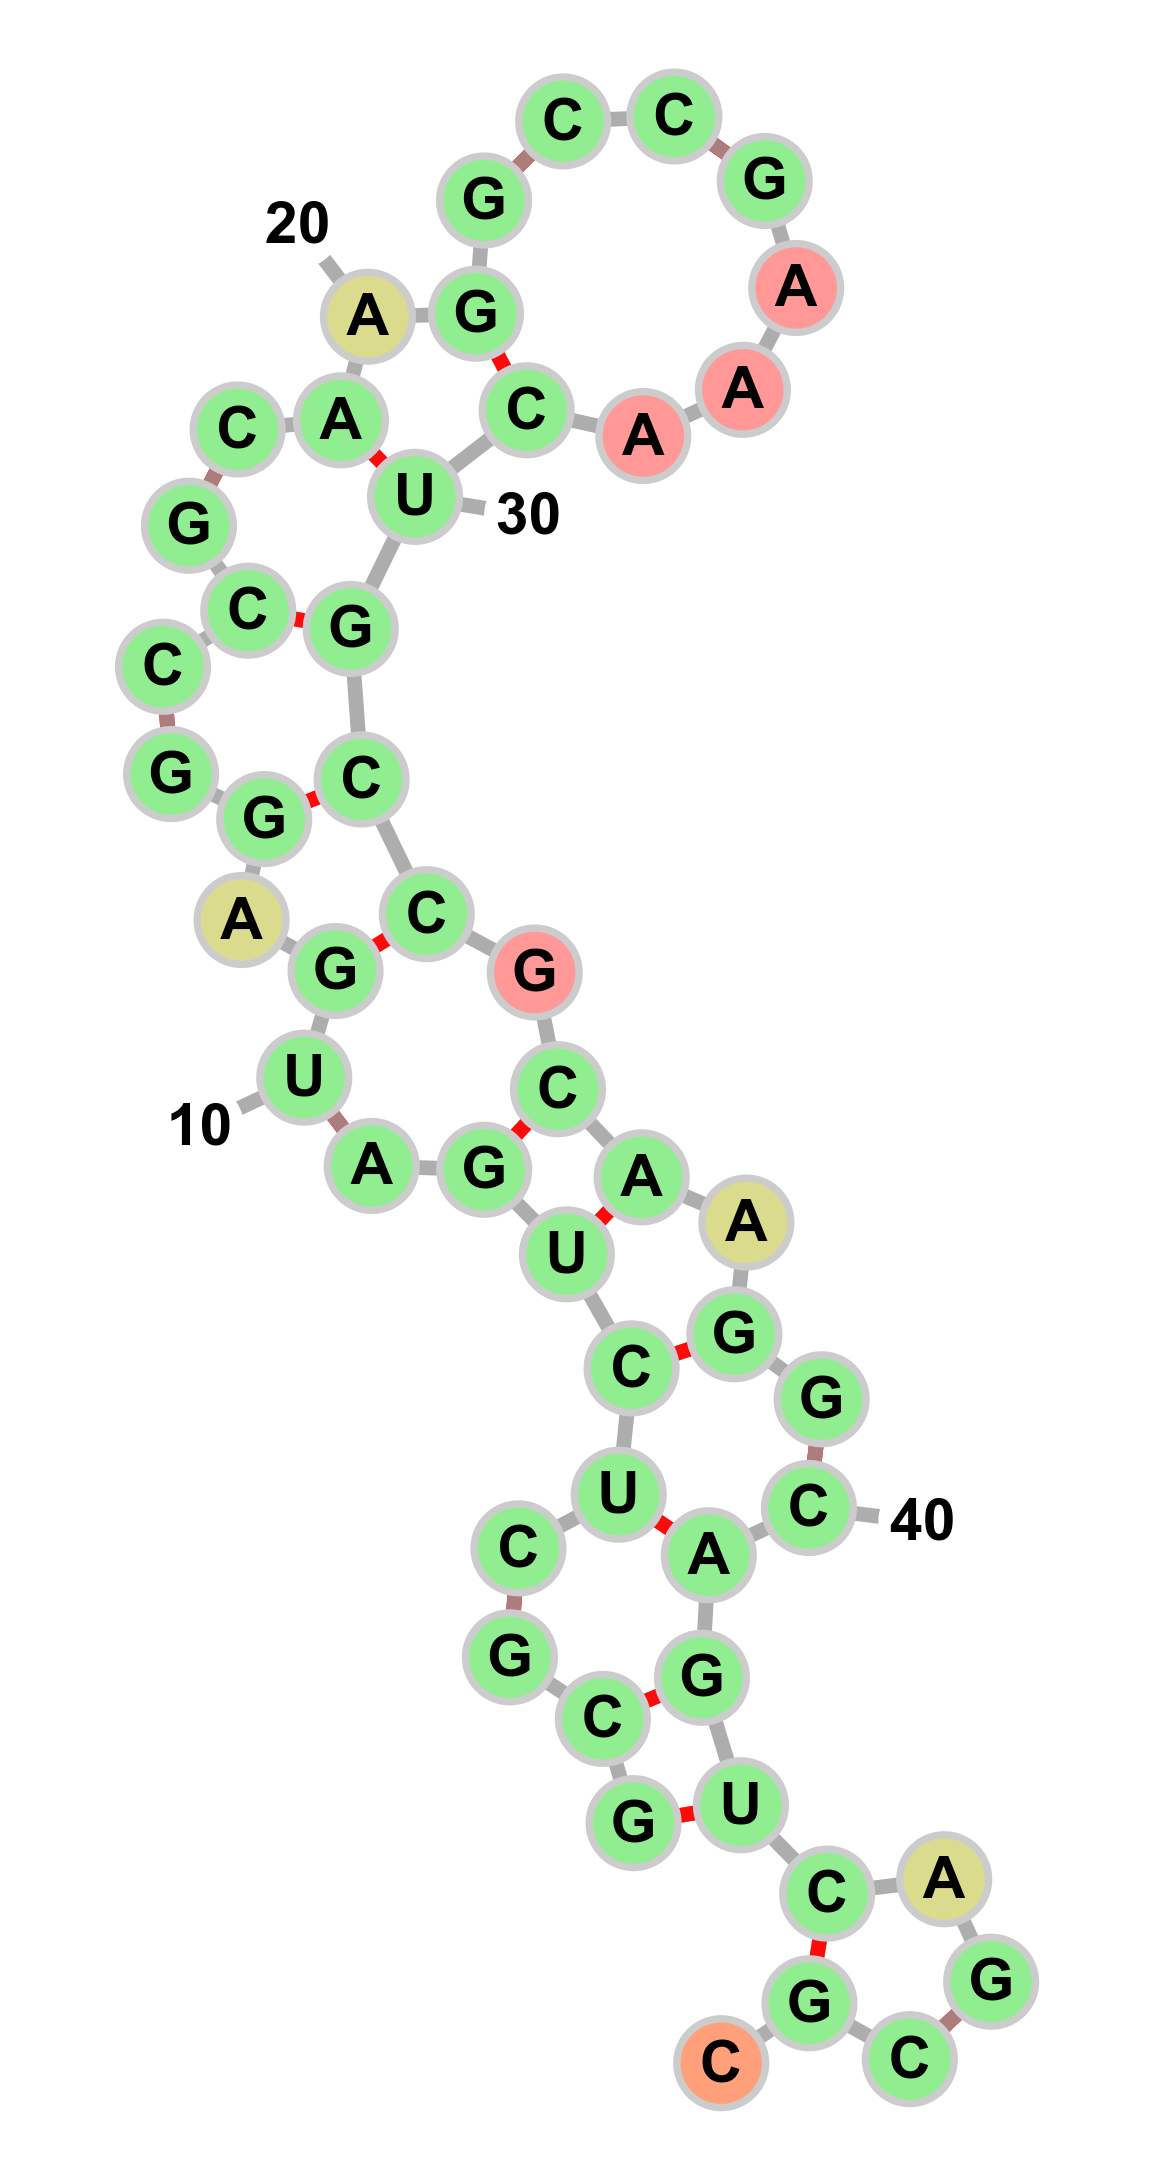
\includegraphics[width=\linewidth]{./img/hammerhead_ribozyme_nussinov.png}
        \caption{Nussinov}
    \end{subfigure}
    \begin{subfigure}[b]{0.4\linewidth}
        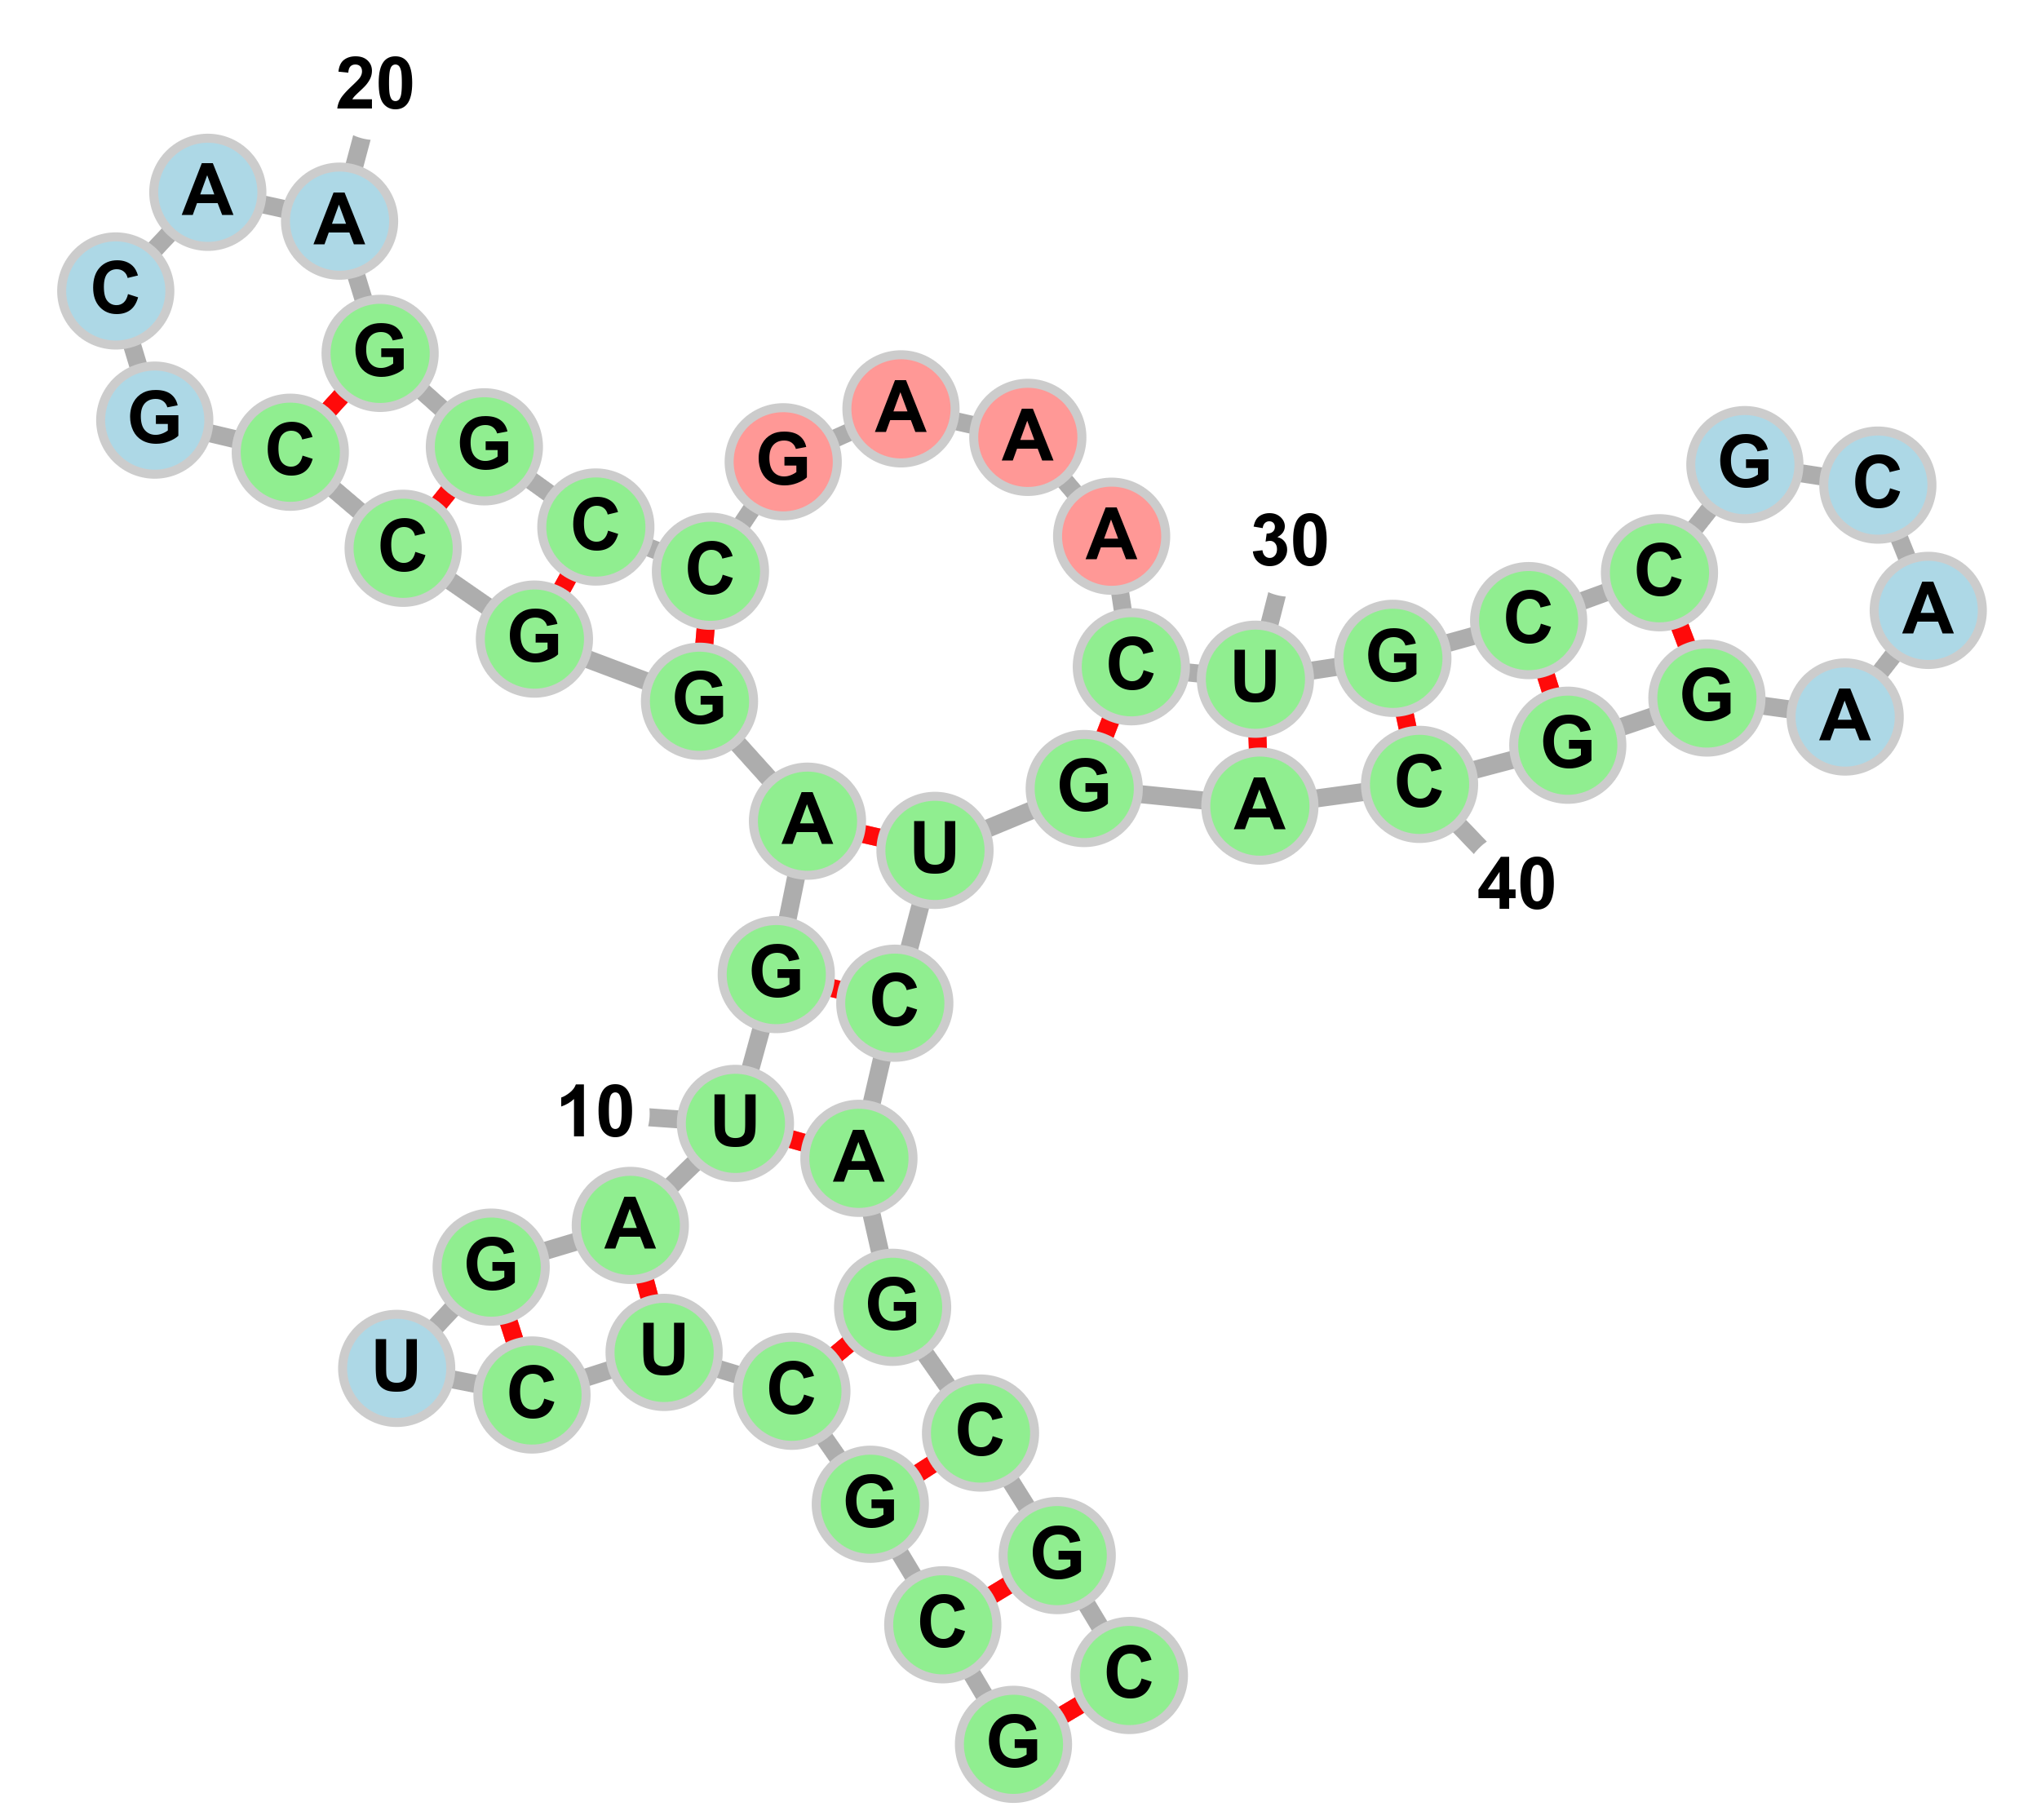
\includegraphics[width=\linewidth]{./img/hammerhead_ribozyme_maxstacks.png}
        \caption{Maximize stacking pairs}
    \end{subfigure}
    \begin{subfigure}[b]{0.4\linewidth}
        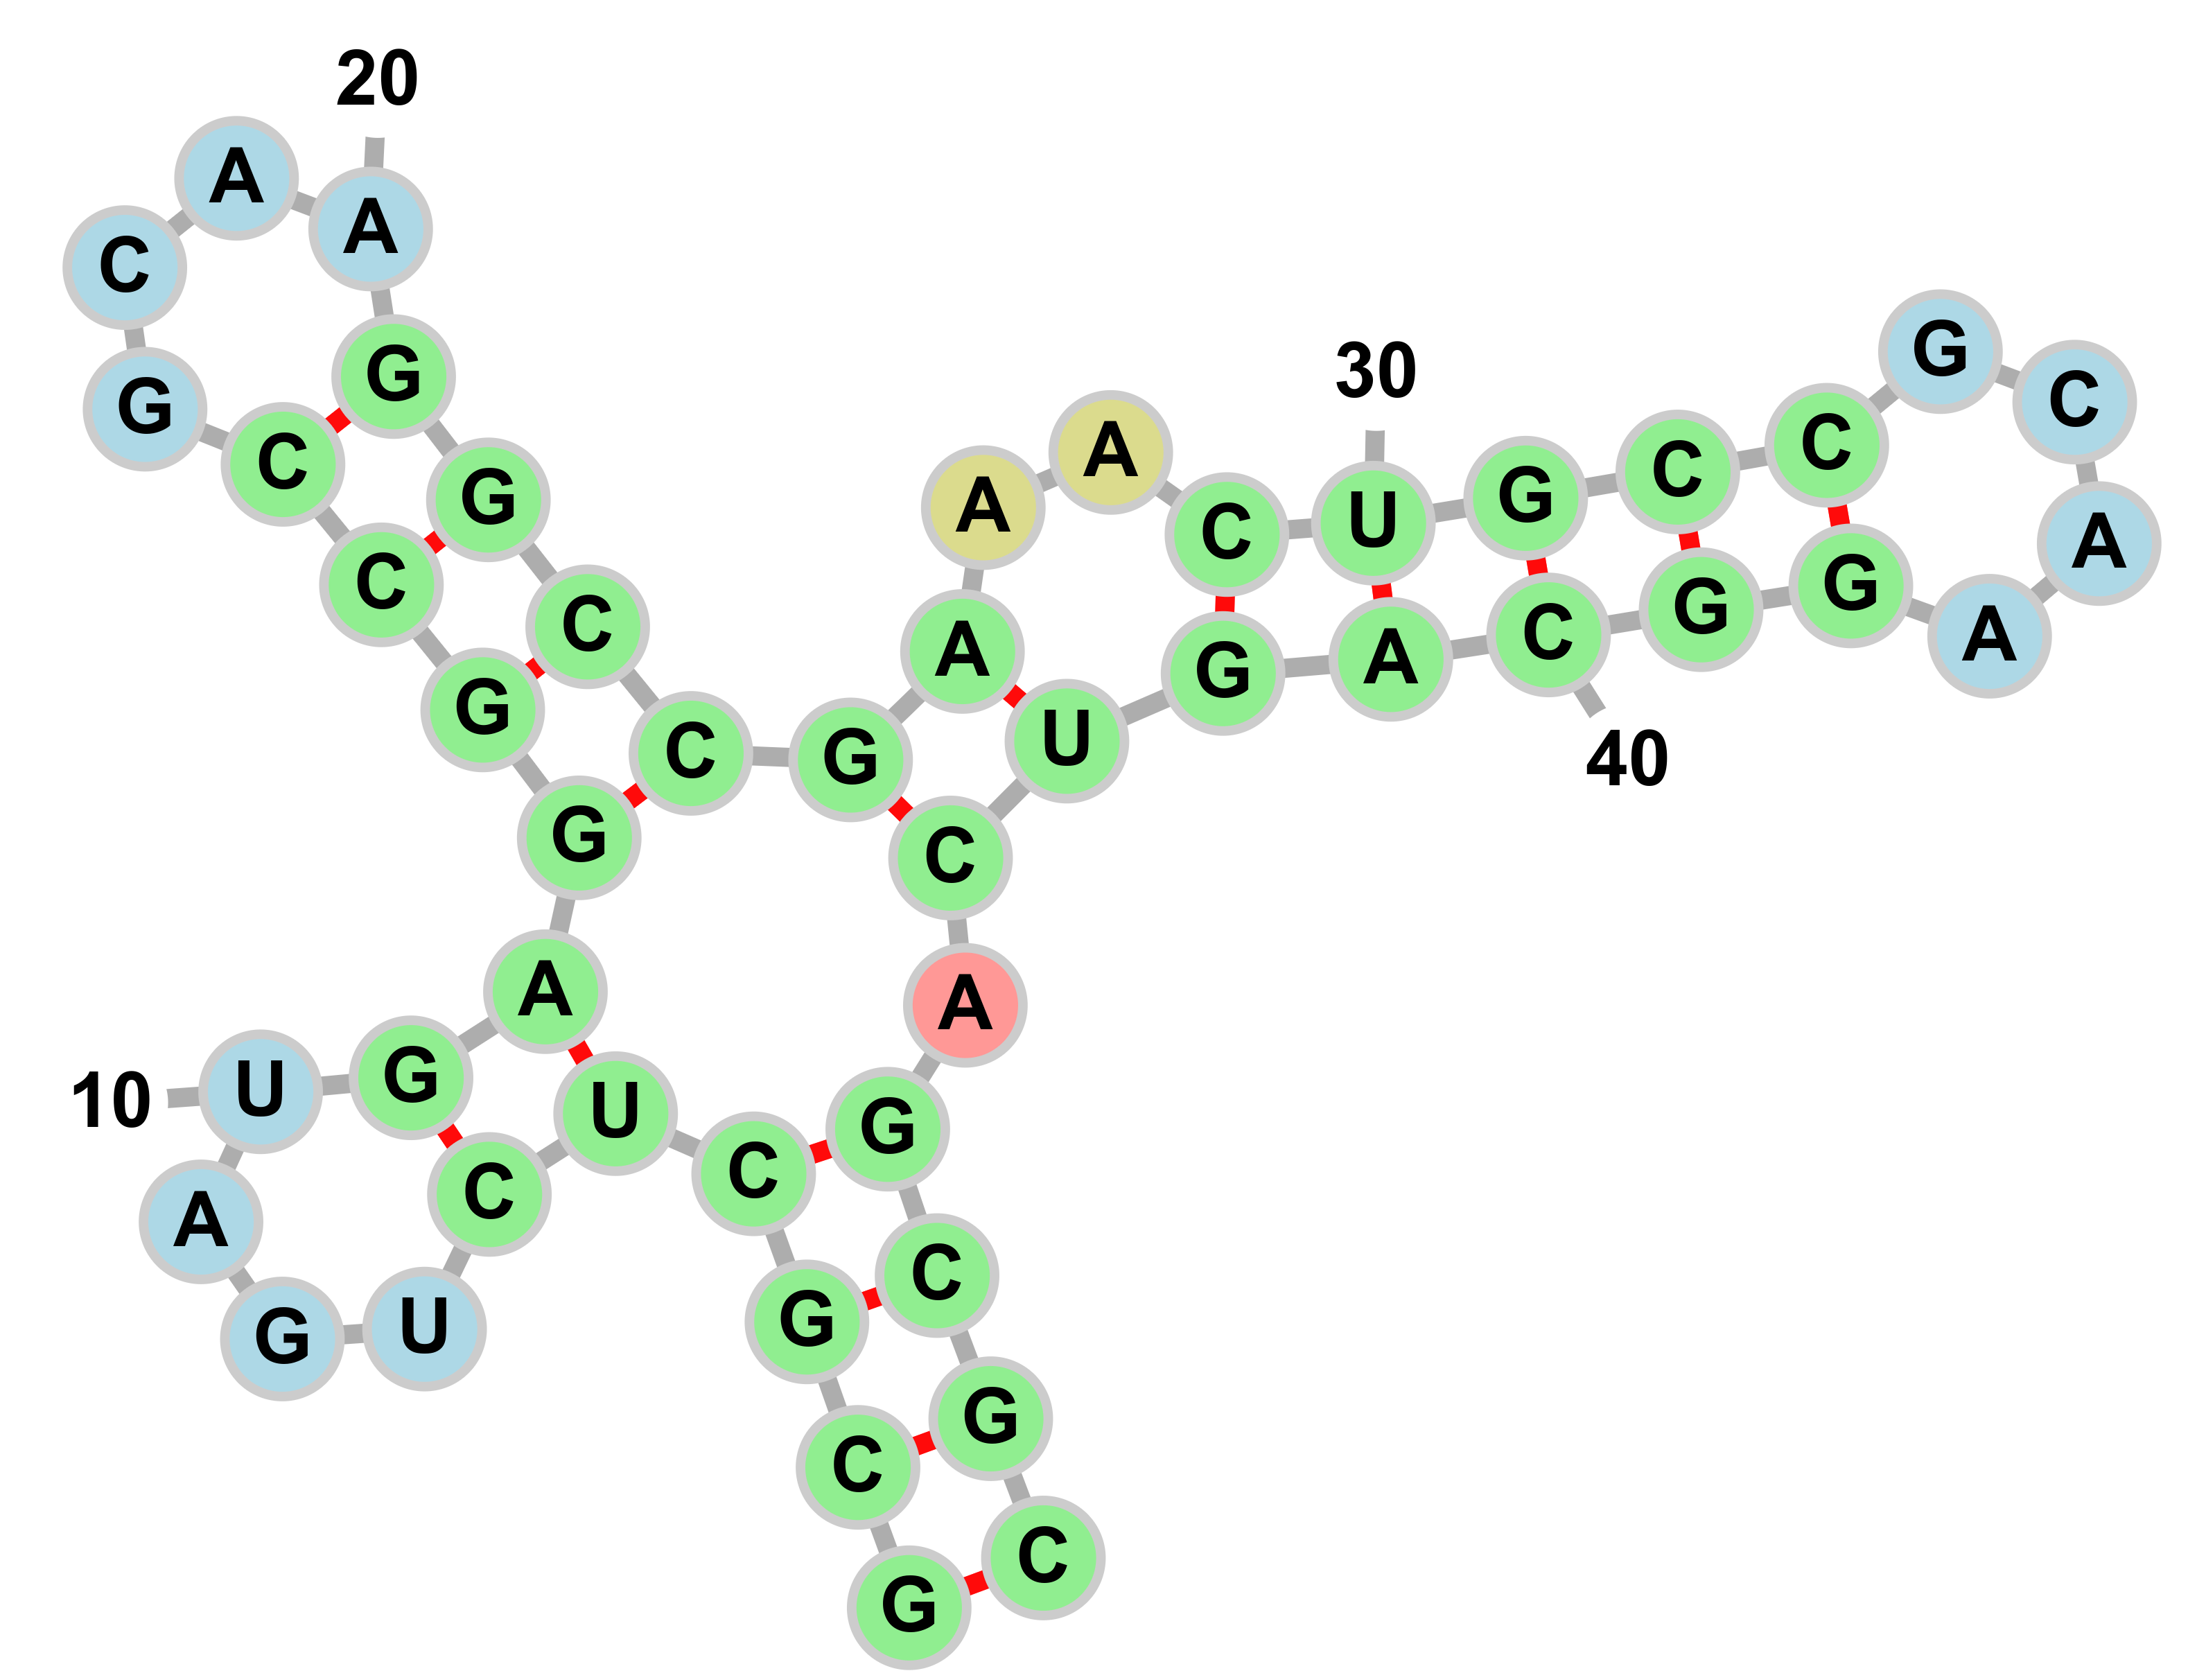
\includegraphics[width=\linewidth]{./img/hammerhead_ribozyme_minstackenergy.png}
        \caption{Minimize stacking pairs energy}
    \end{subfigure}
    \begin{center}
        \begin{subfigure}[b]{0.5\linewidth}
            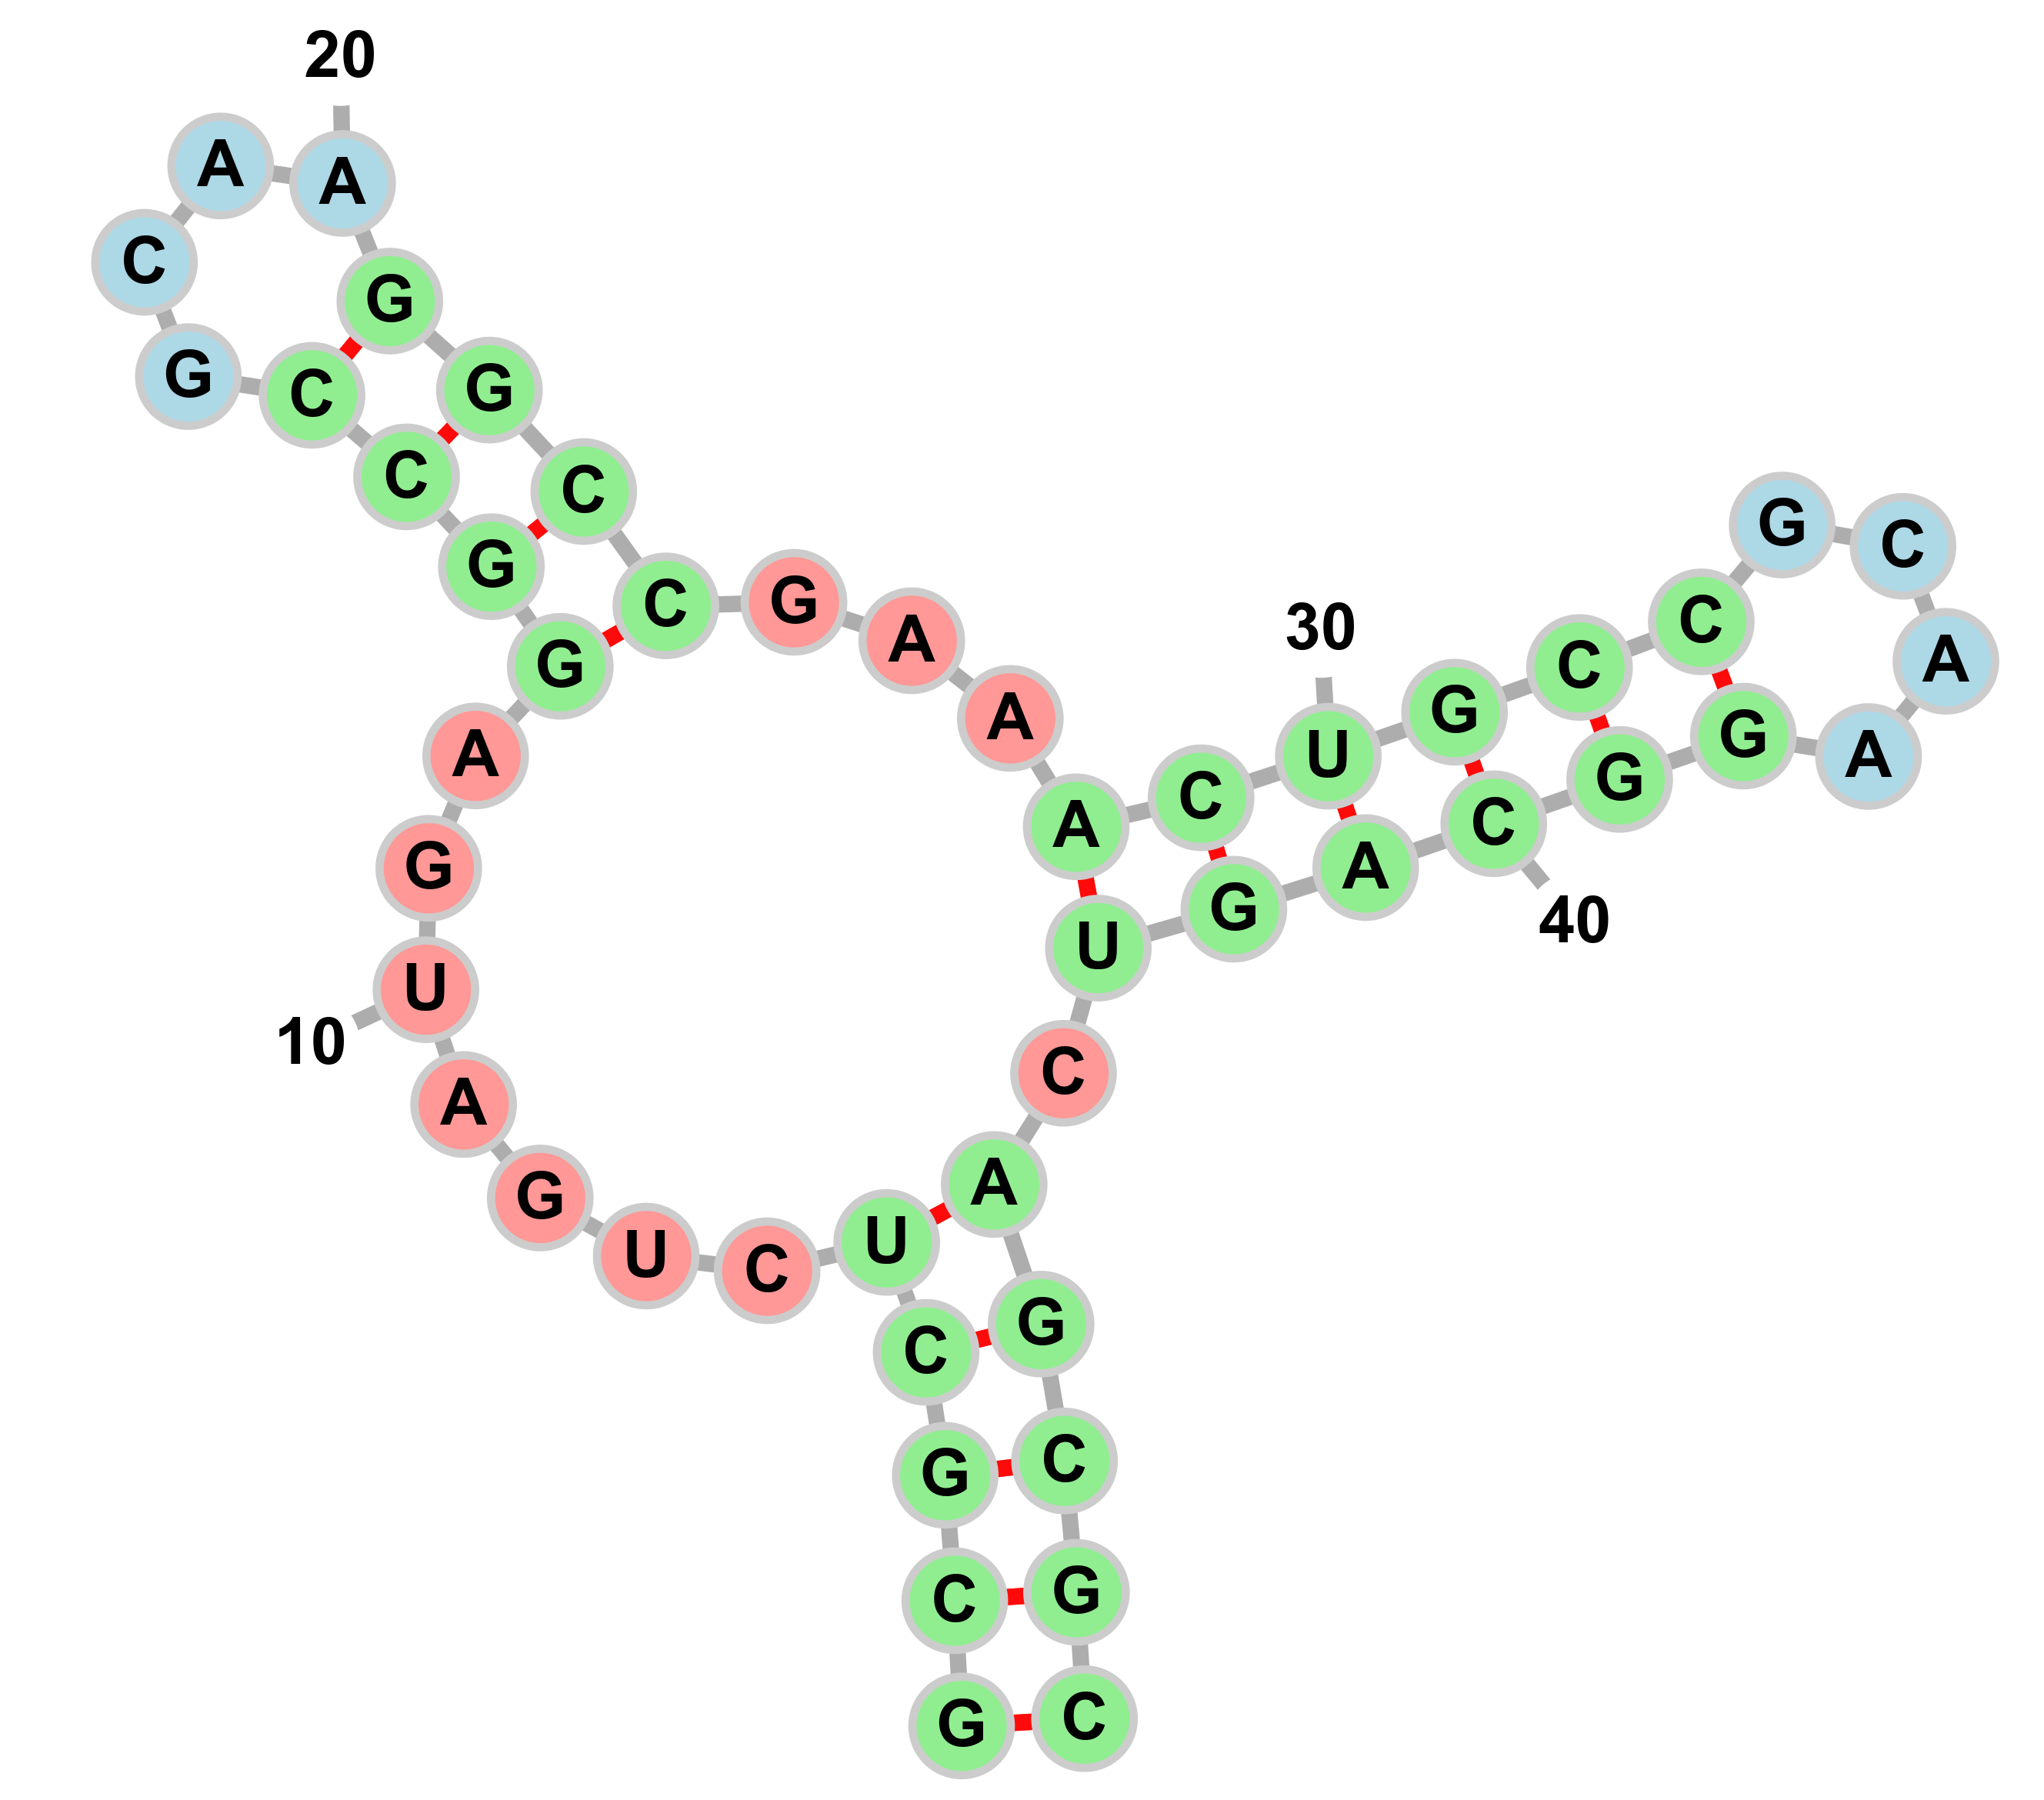
\includegraphics[width=\linewidth]{./img/hammerhead_ribozyme_correct.png}
            \caption{Correct}
        \end{subfigure}
    \end{center}
\caption{hammerhead ribozyme}
\label{fig:harmmerhead}
\end{figure}

\begin{figure}[p]
    \begin{subfigure}[b]{0.2\linewidth}
        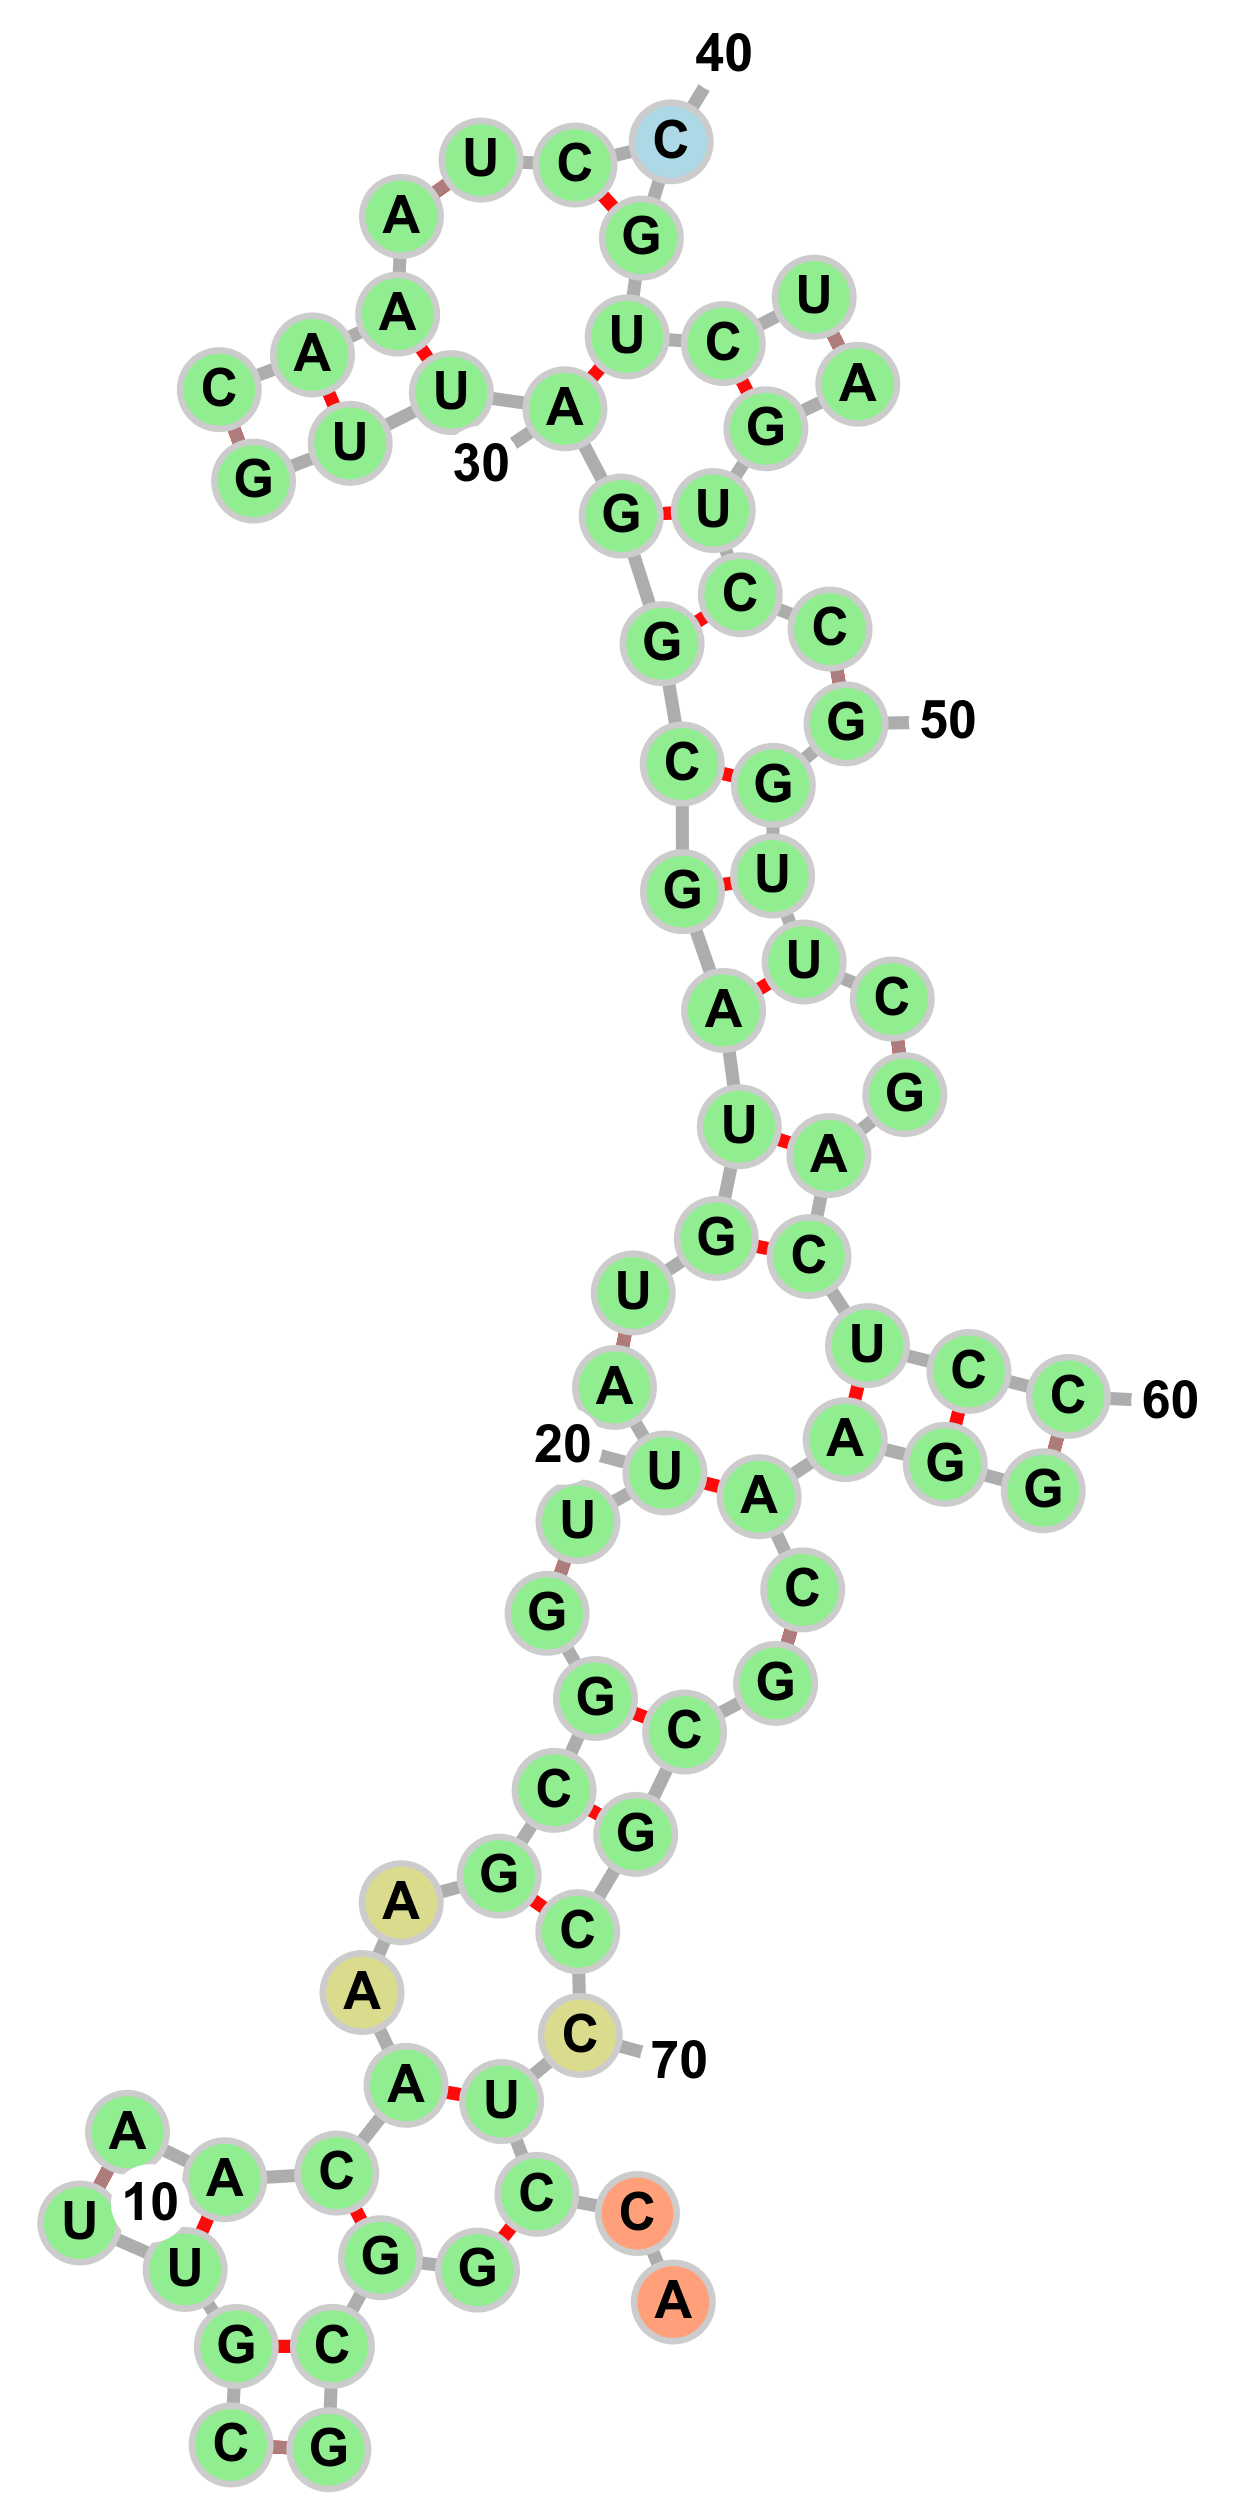
\includegraphics[width=\linewidth]{./img/PDB_00313_nussinov.png}
        \caption{Nussinov}
    \end{subfigure}
    \begin{subfigure}[b]{0.4\linewidth}
        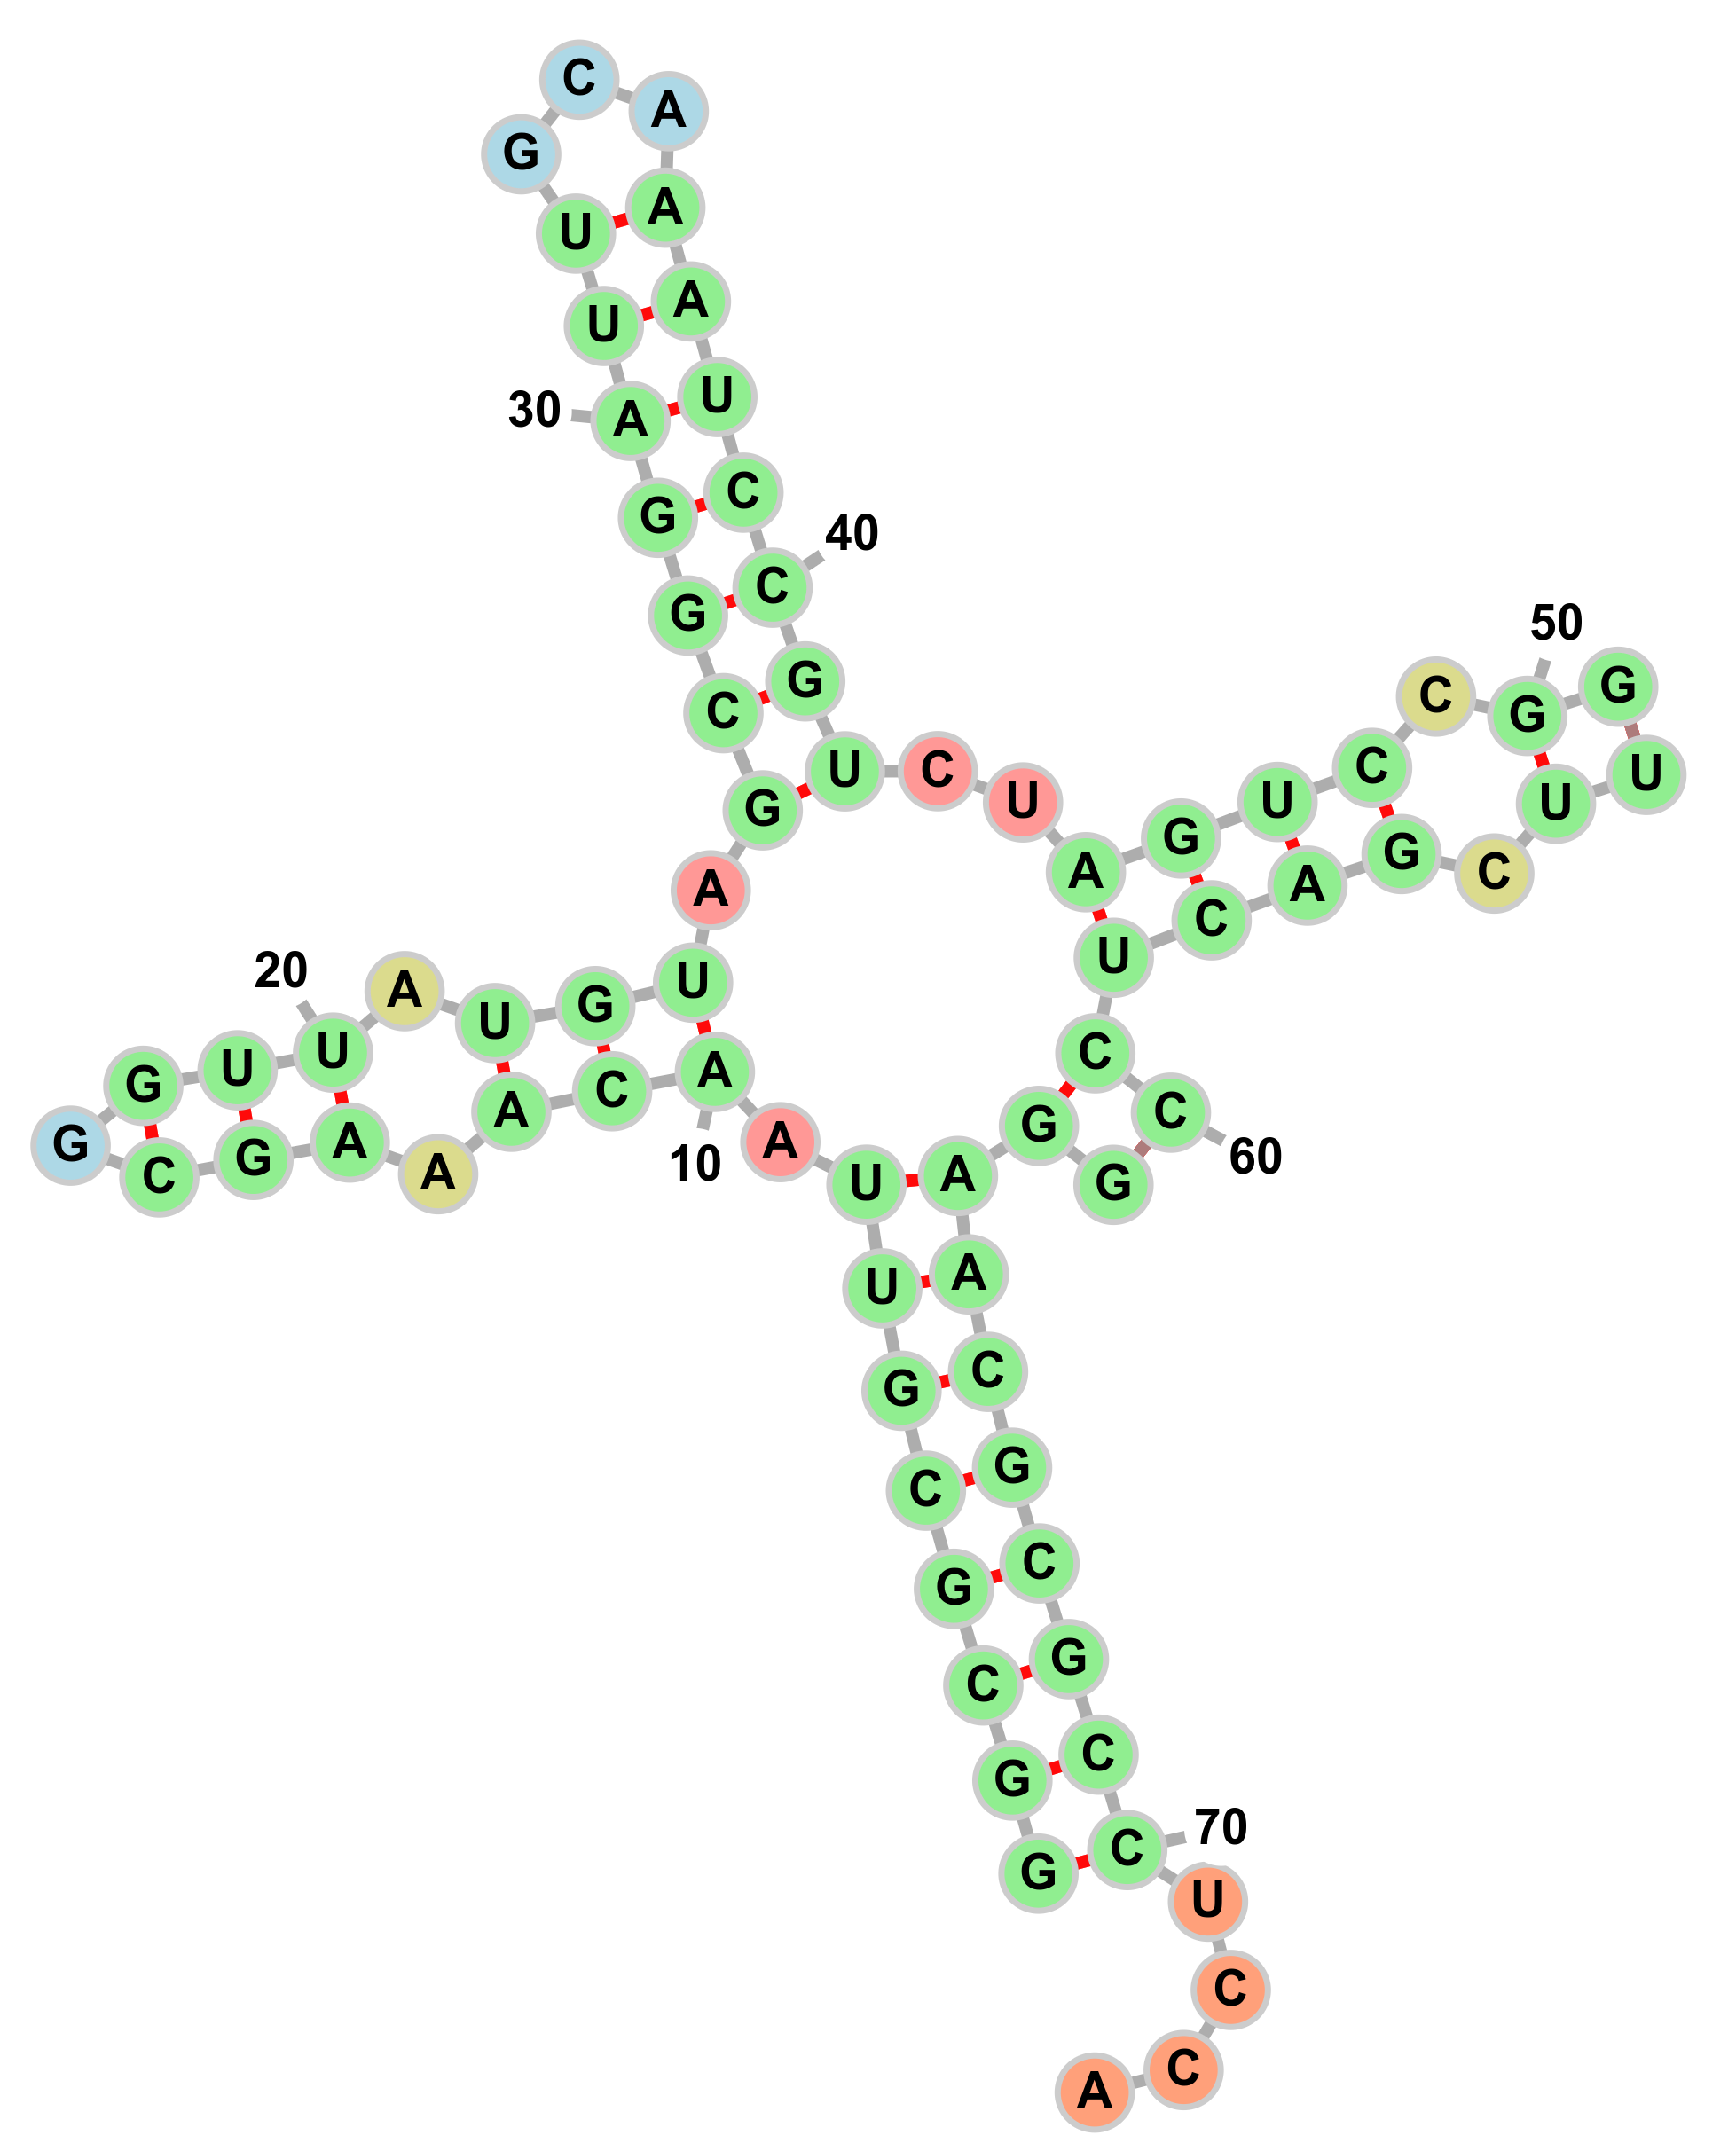
\includegraphics[width=\linewidth]{./img/PDB_00313_maxstacks.png}
        \caption{Maximize stacking pairs}
    \end{subfigure}
    \begin{subfigure}[b]{0.4\linewidth}
        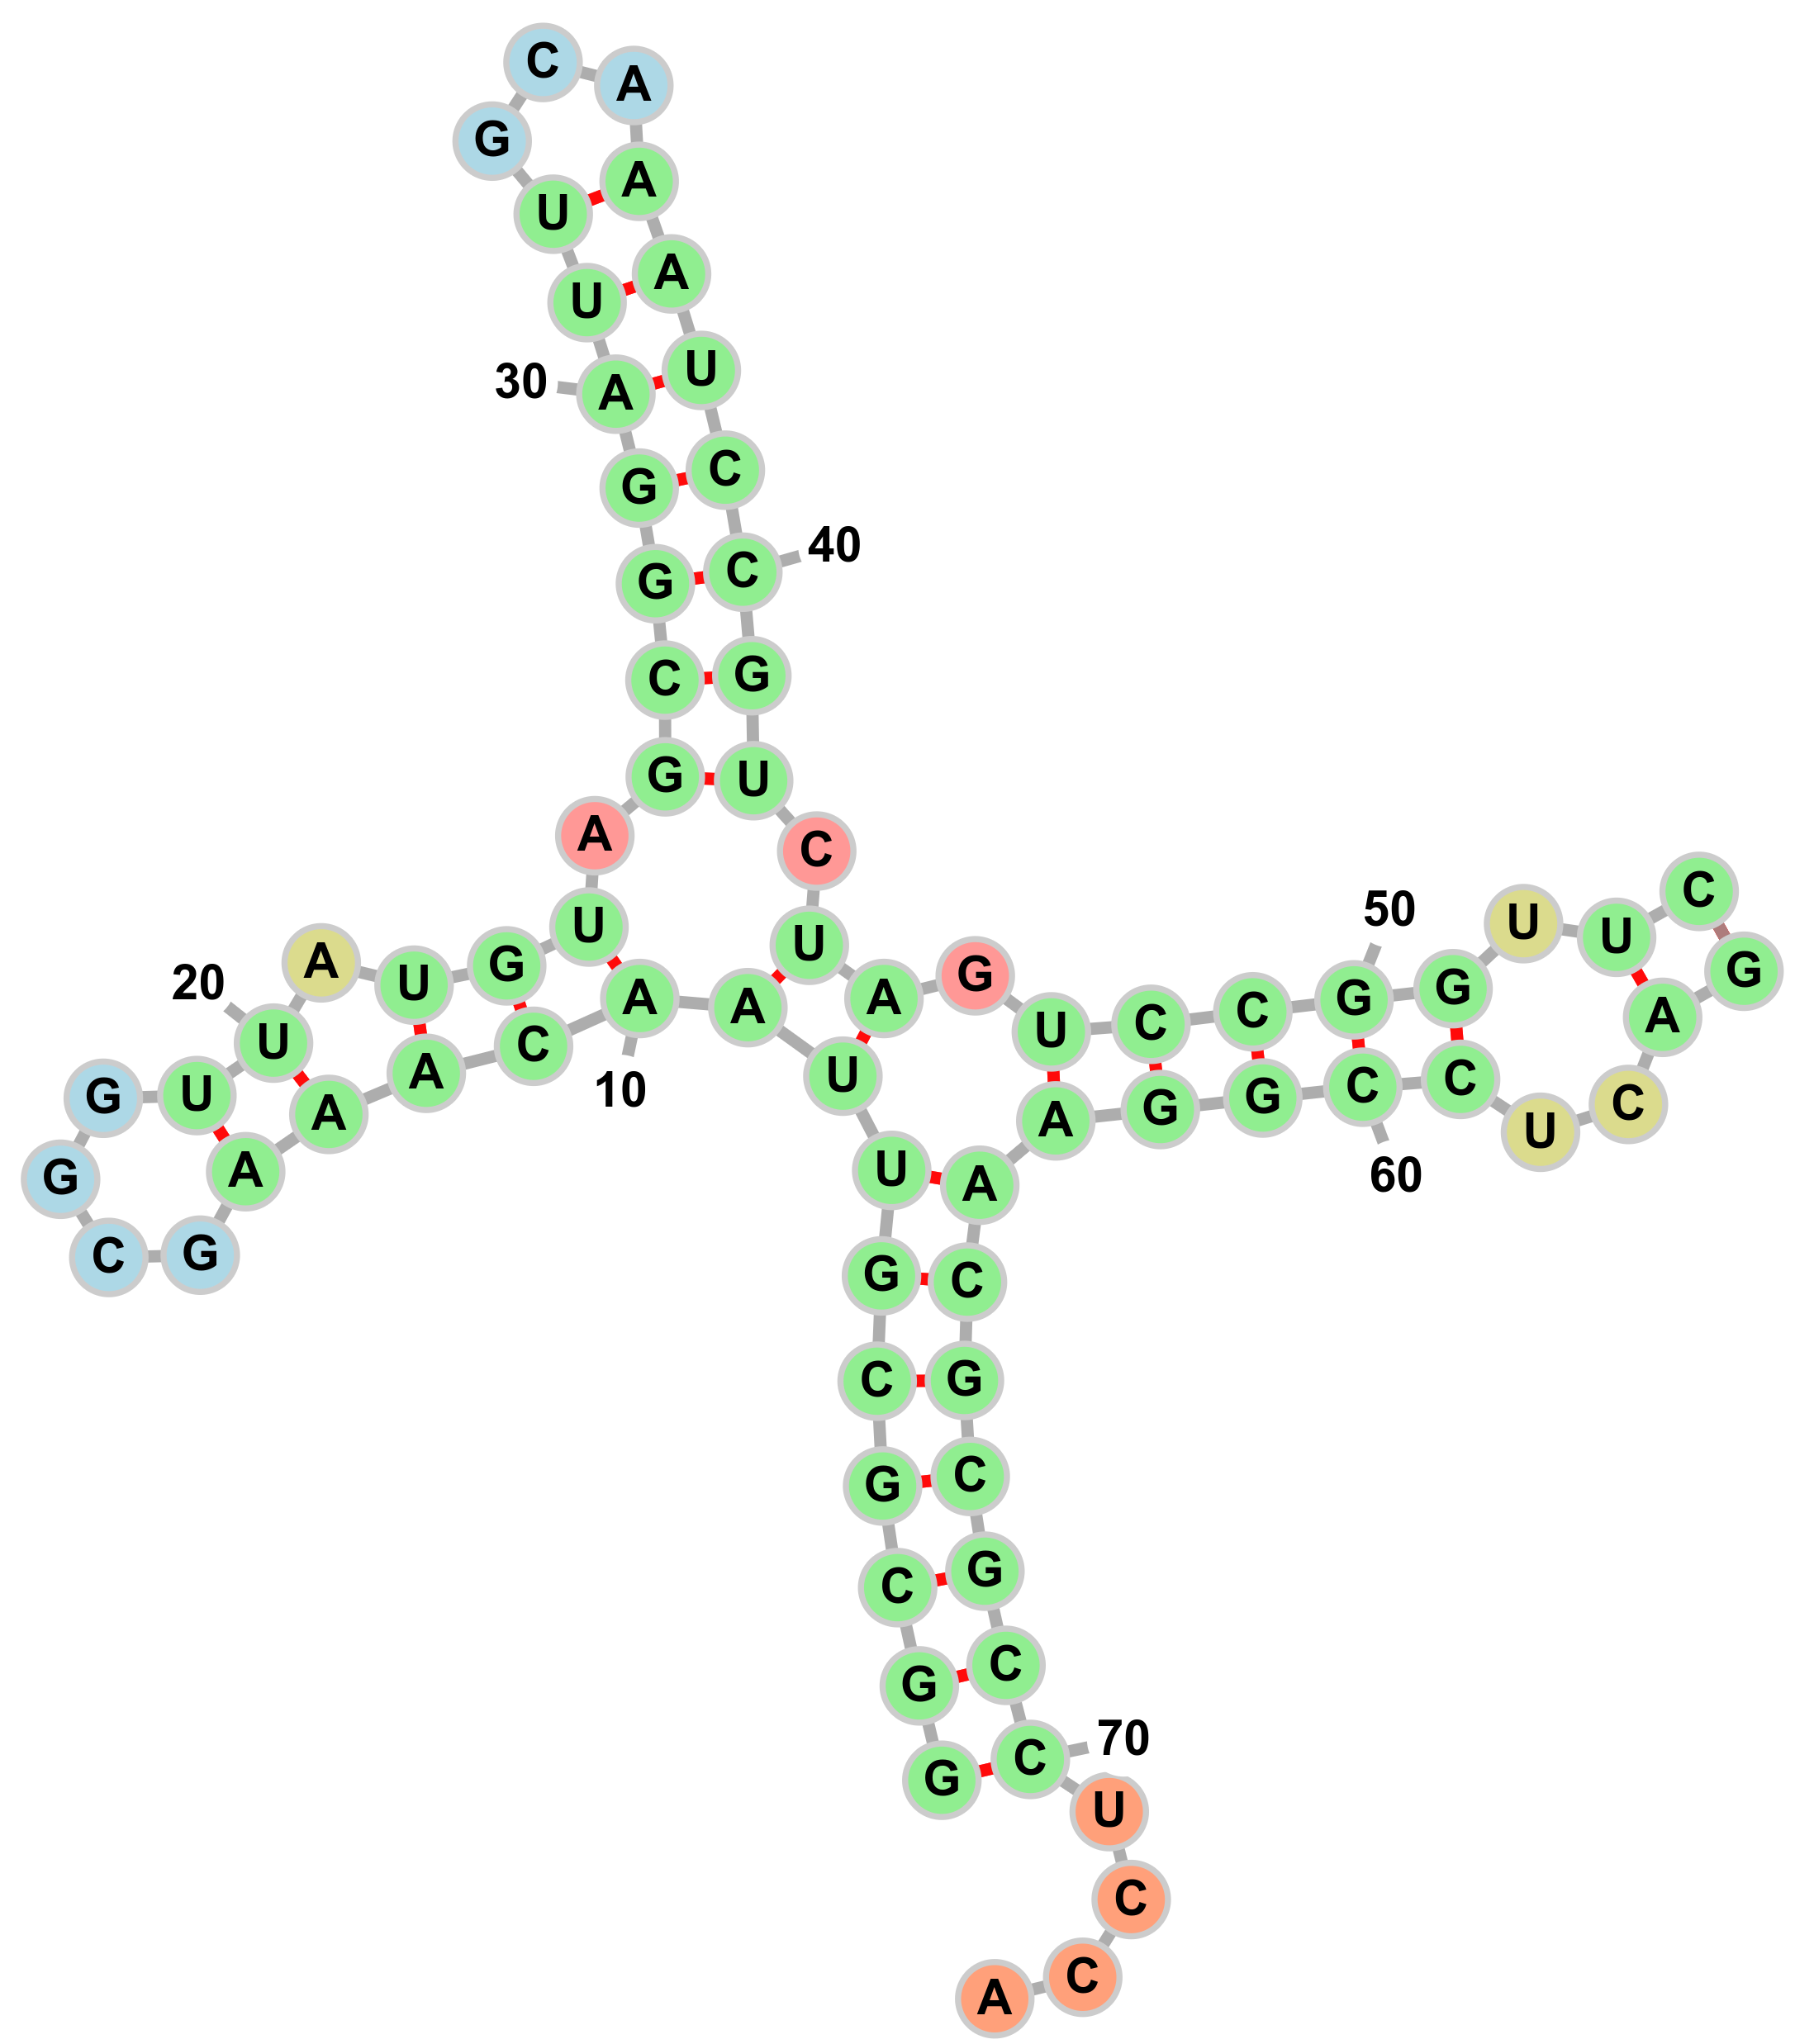
\includegraphics[width=\linewidth]{./img/PDB_00313_minstackenergy.png}
        \caption{Minimize stacking pairs energy}
    \end{subfigure}
    \begin{center}
        \begin{subfigure}[b]{0.5\linewidth}
            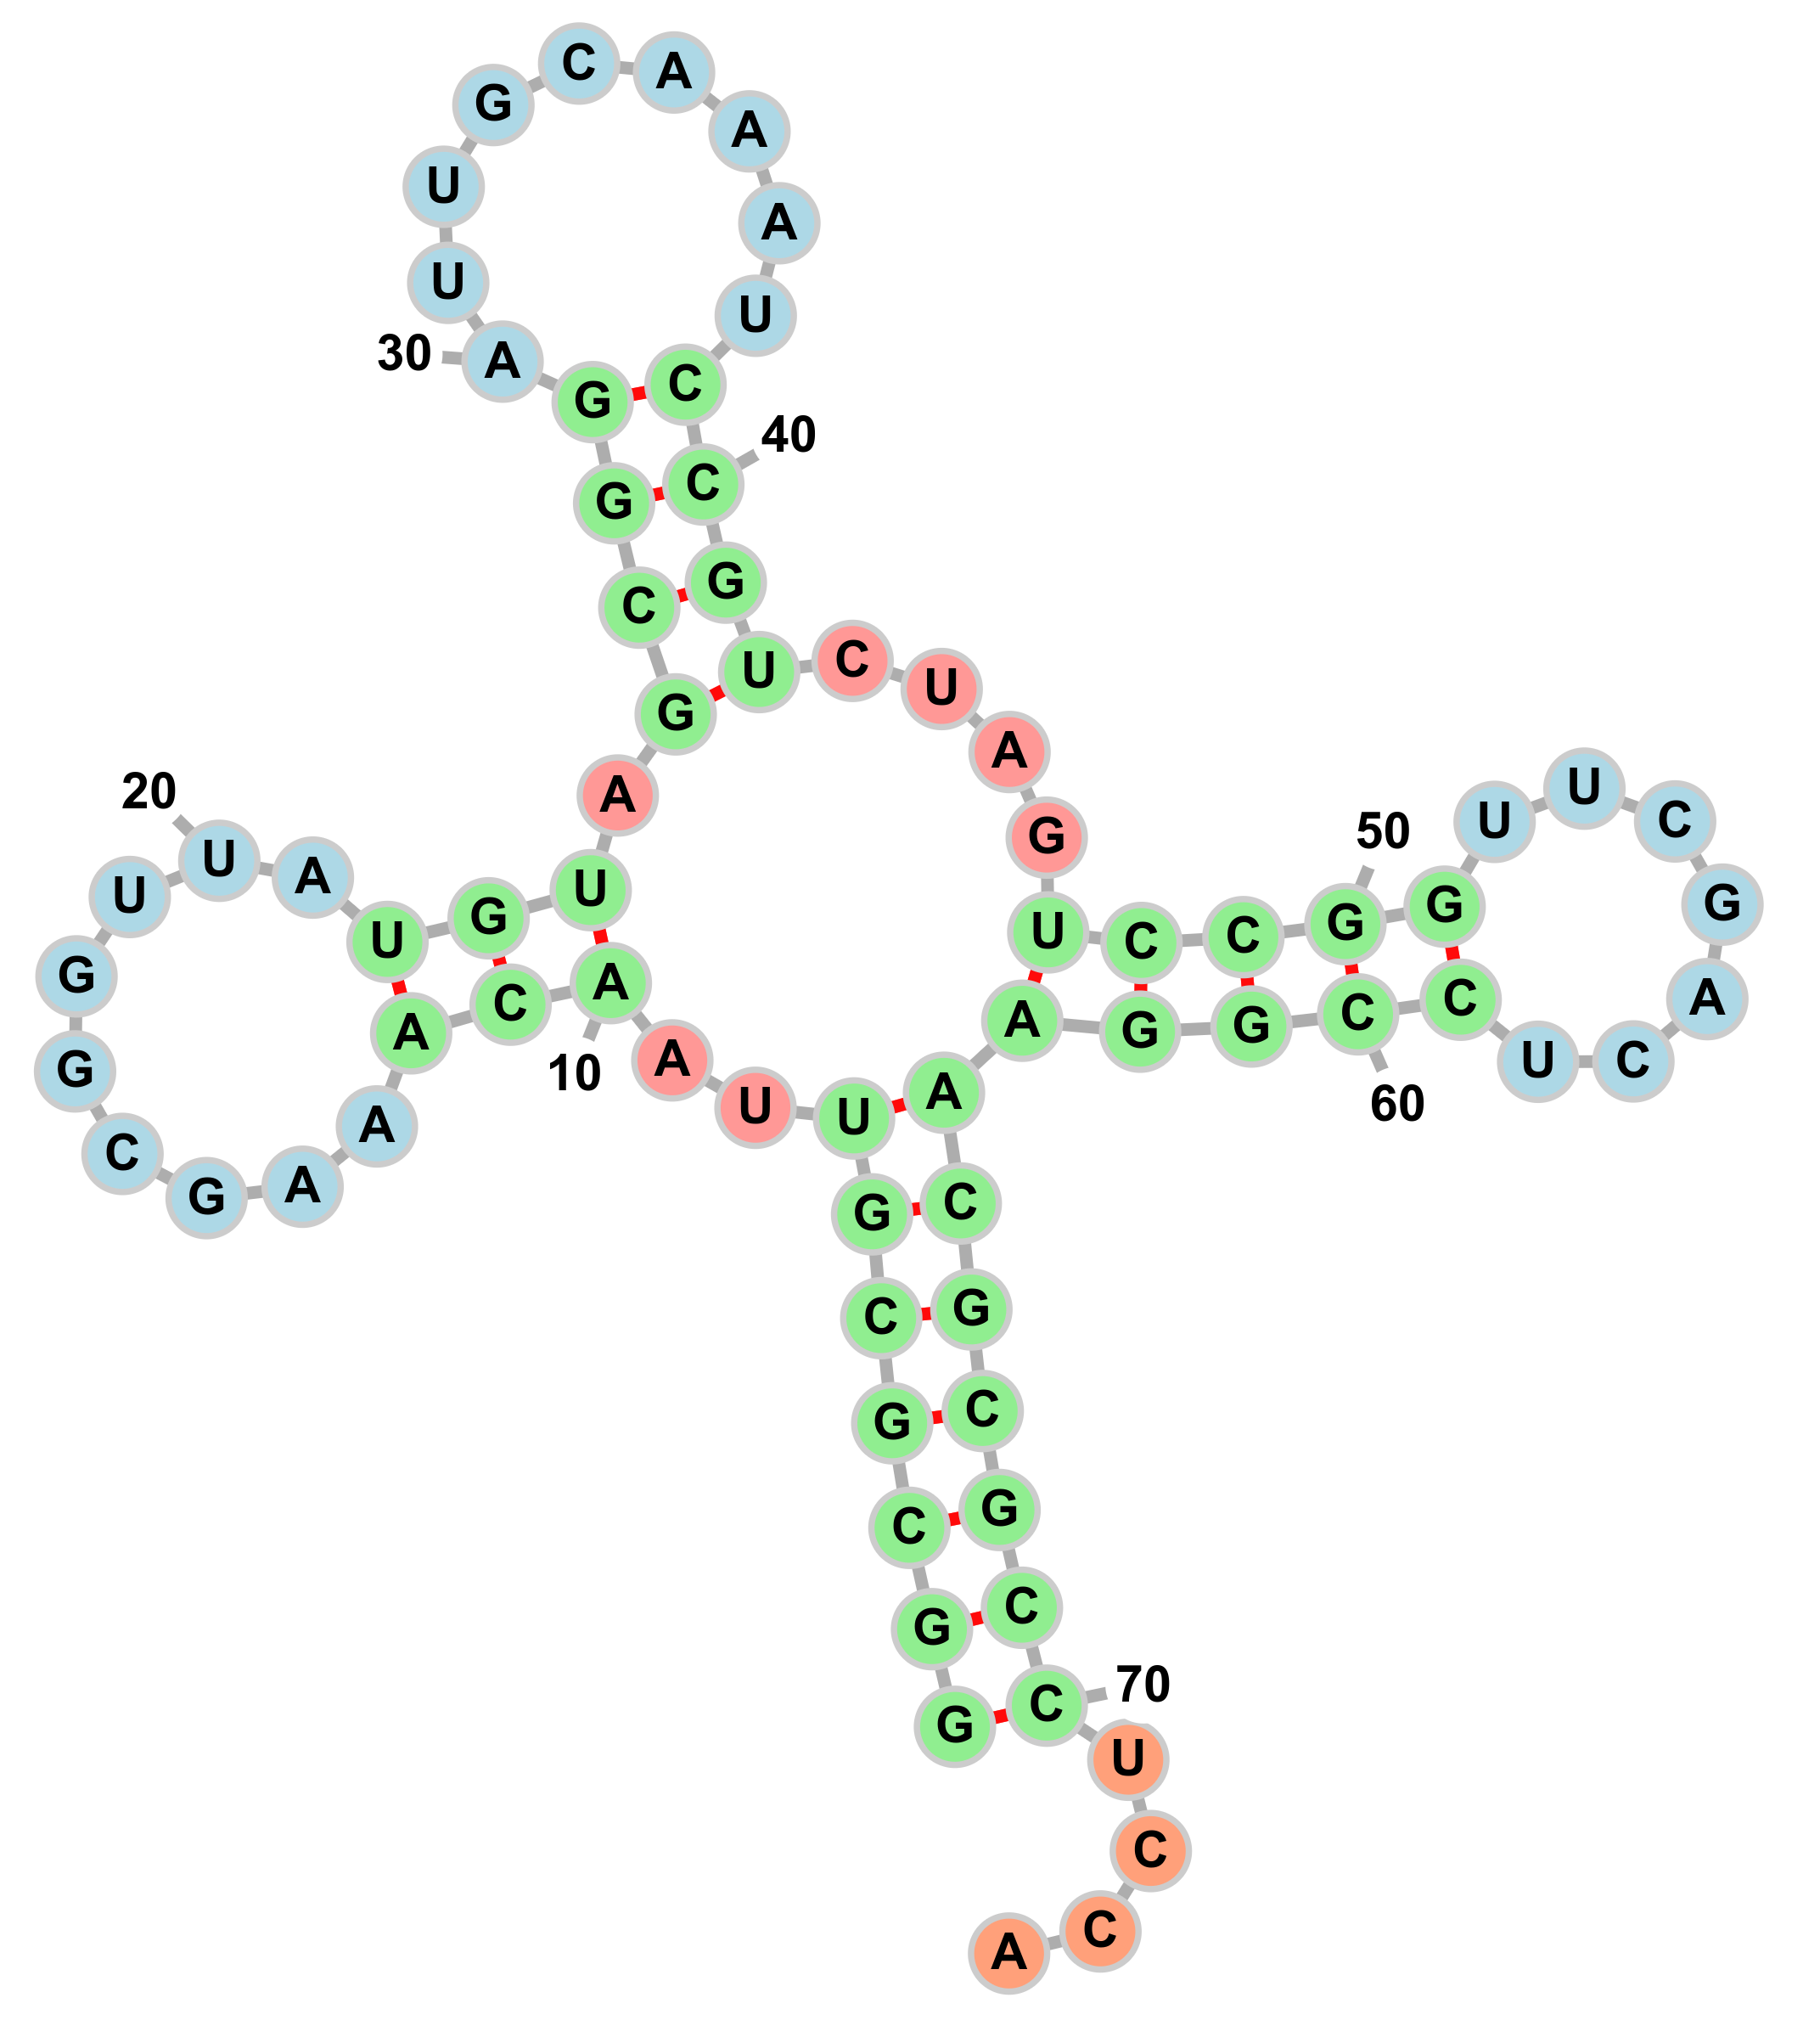
\includegraphics[width=\linewidth]{./img/PDB_00313_correct.png}
            \caption{Correct}
        \end{subfigure}
    \end{center}
\caption{PDB\_00313}
\label{fig:PDB_00313}
\end{figure}

\begin{figure}[p]
    \begin{subfigure}[b]{0.2\linewidth}
        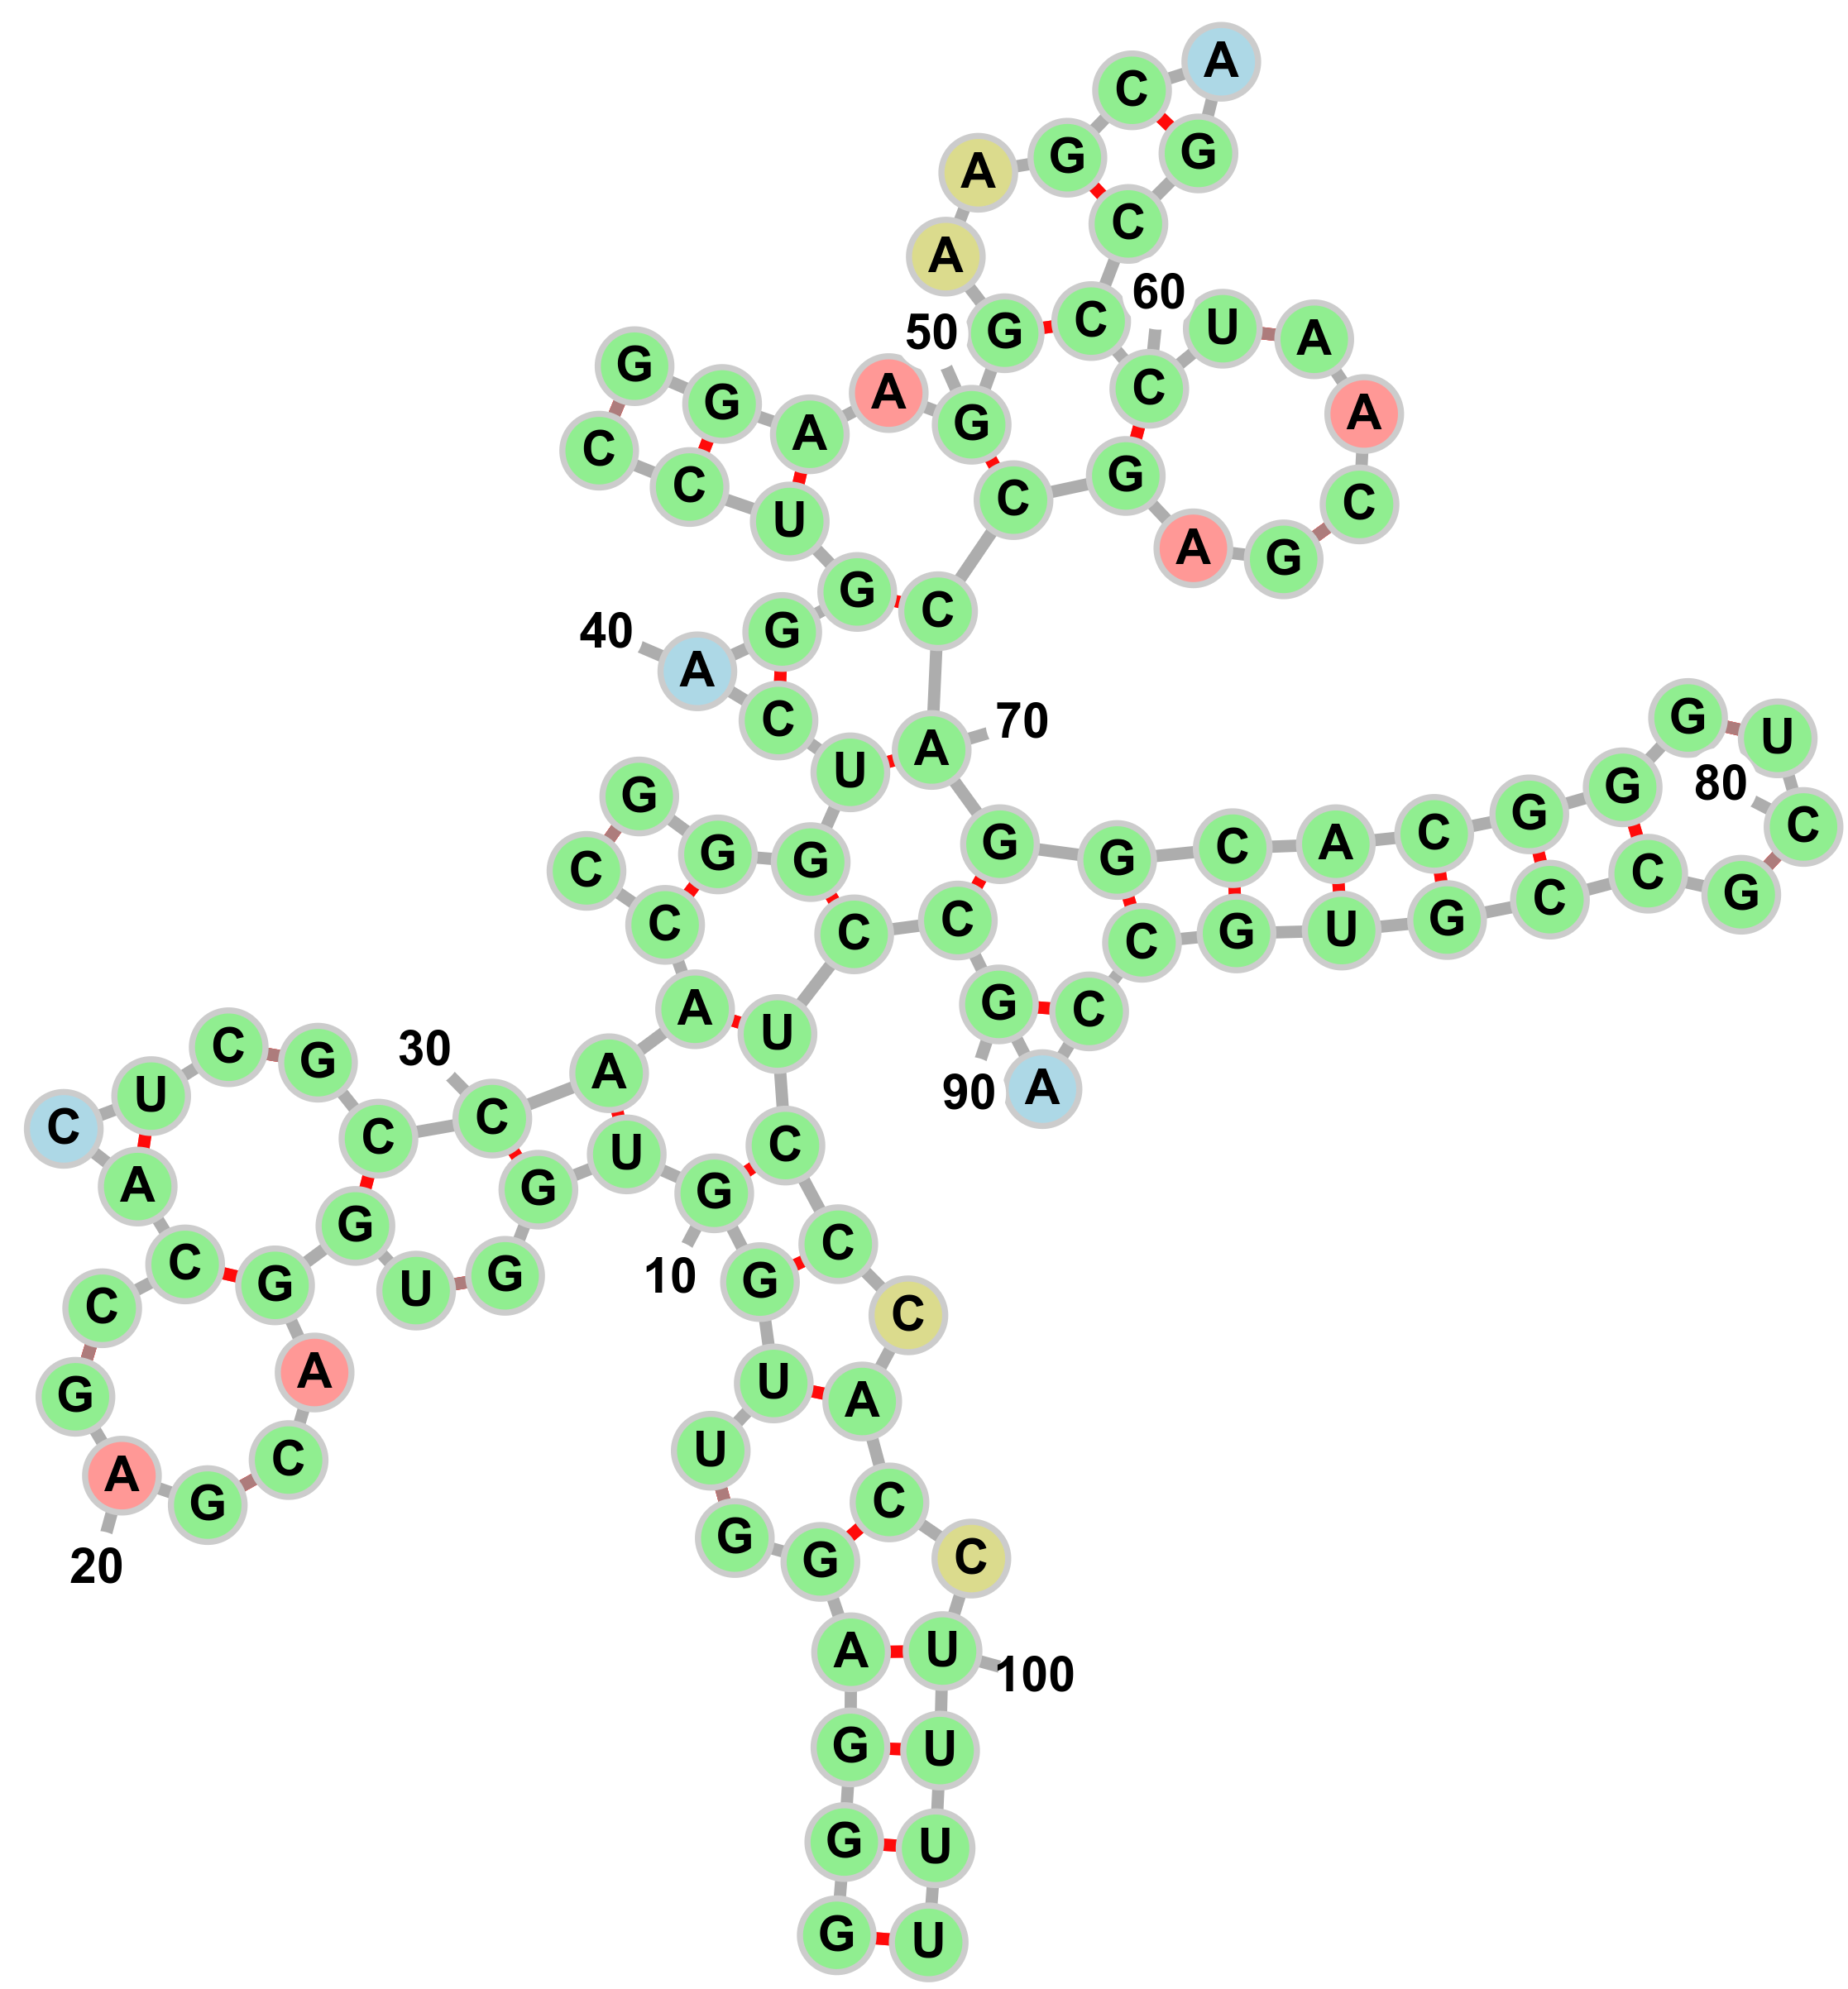
\includegraphics[width=\linewidth]{./img/SRP_00004_nussinov.png}
        \caption{Nussinov}
    \end{subfigure}
    \begin{subfigure}[b]{0.4\linewidth}
        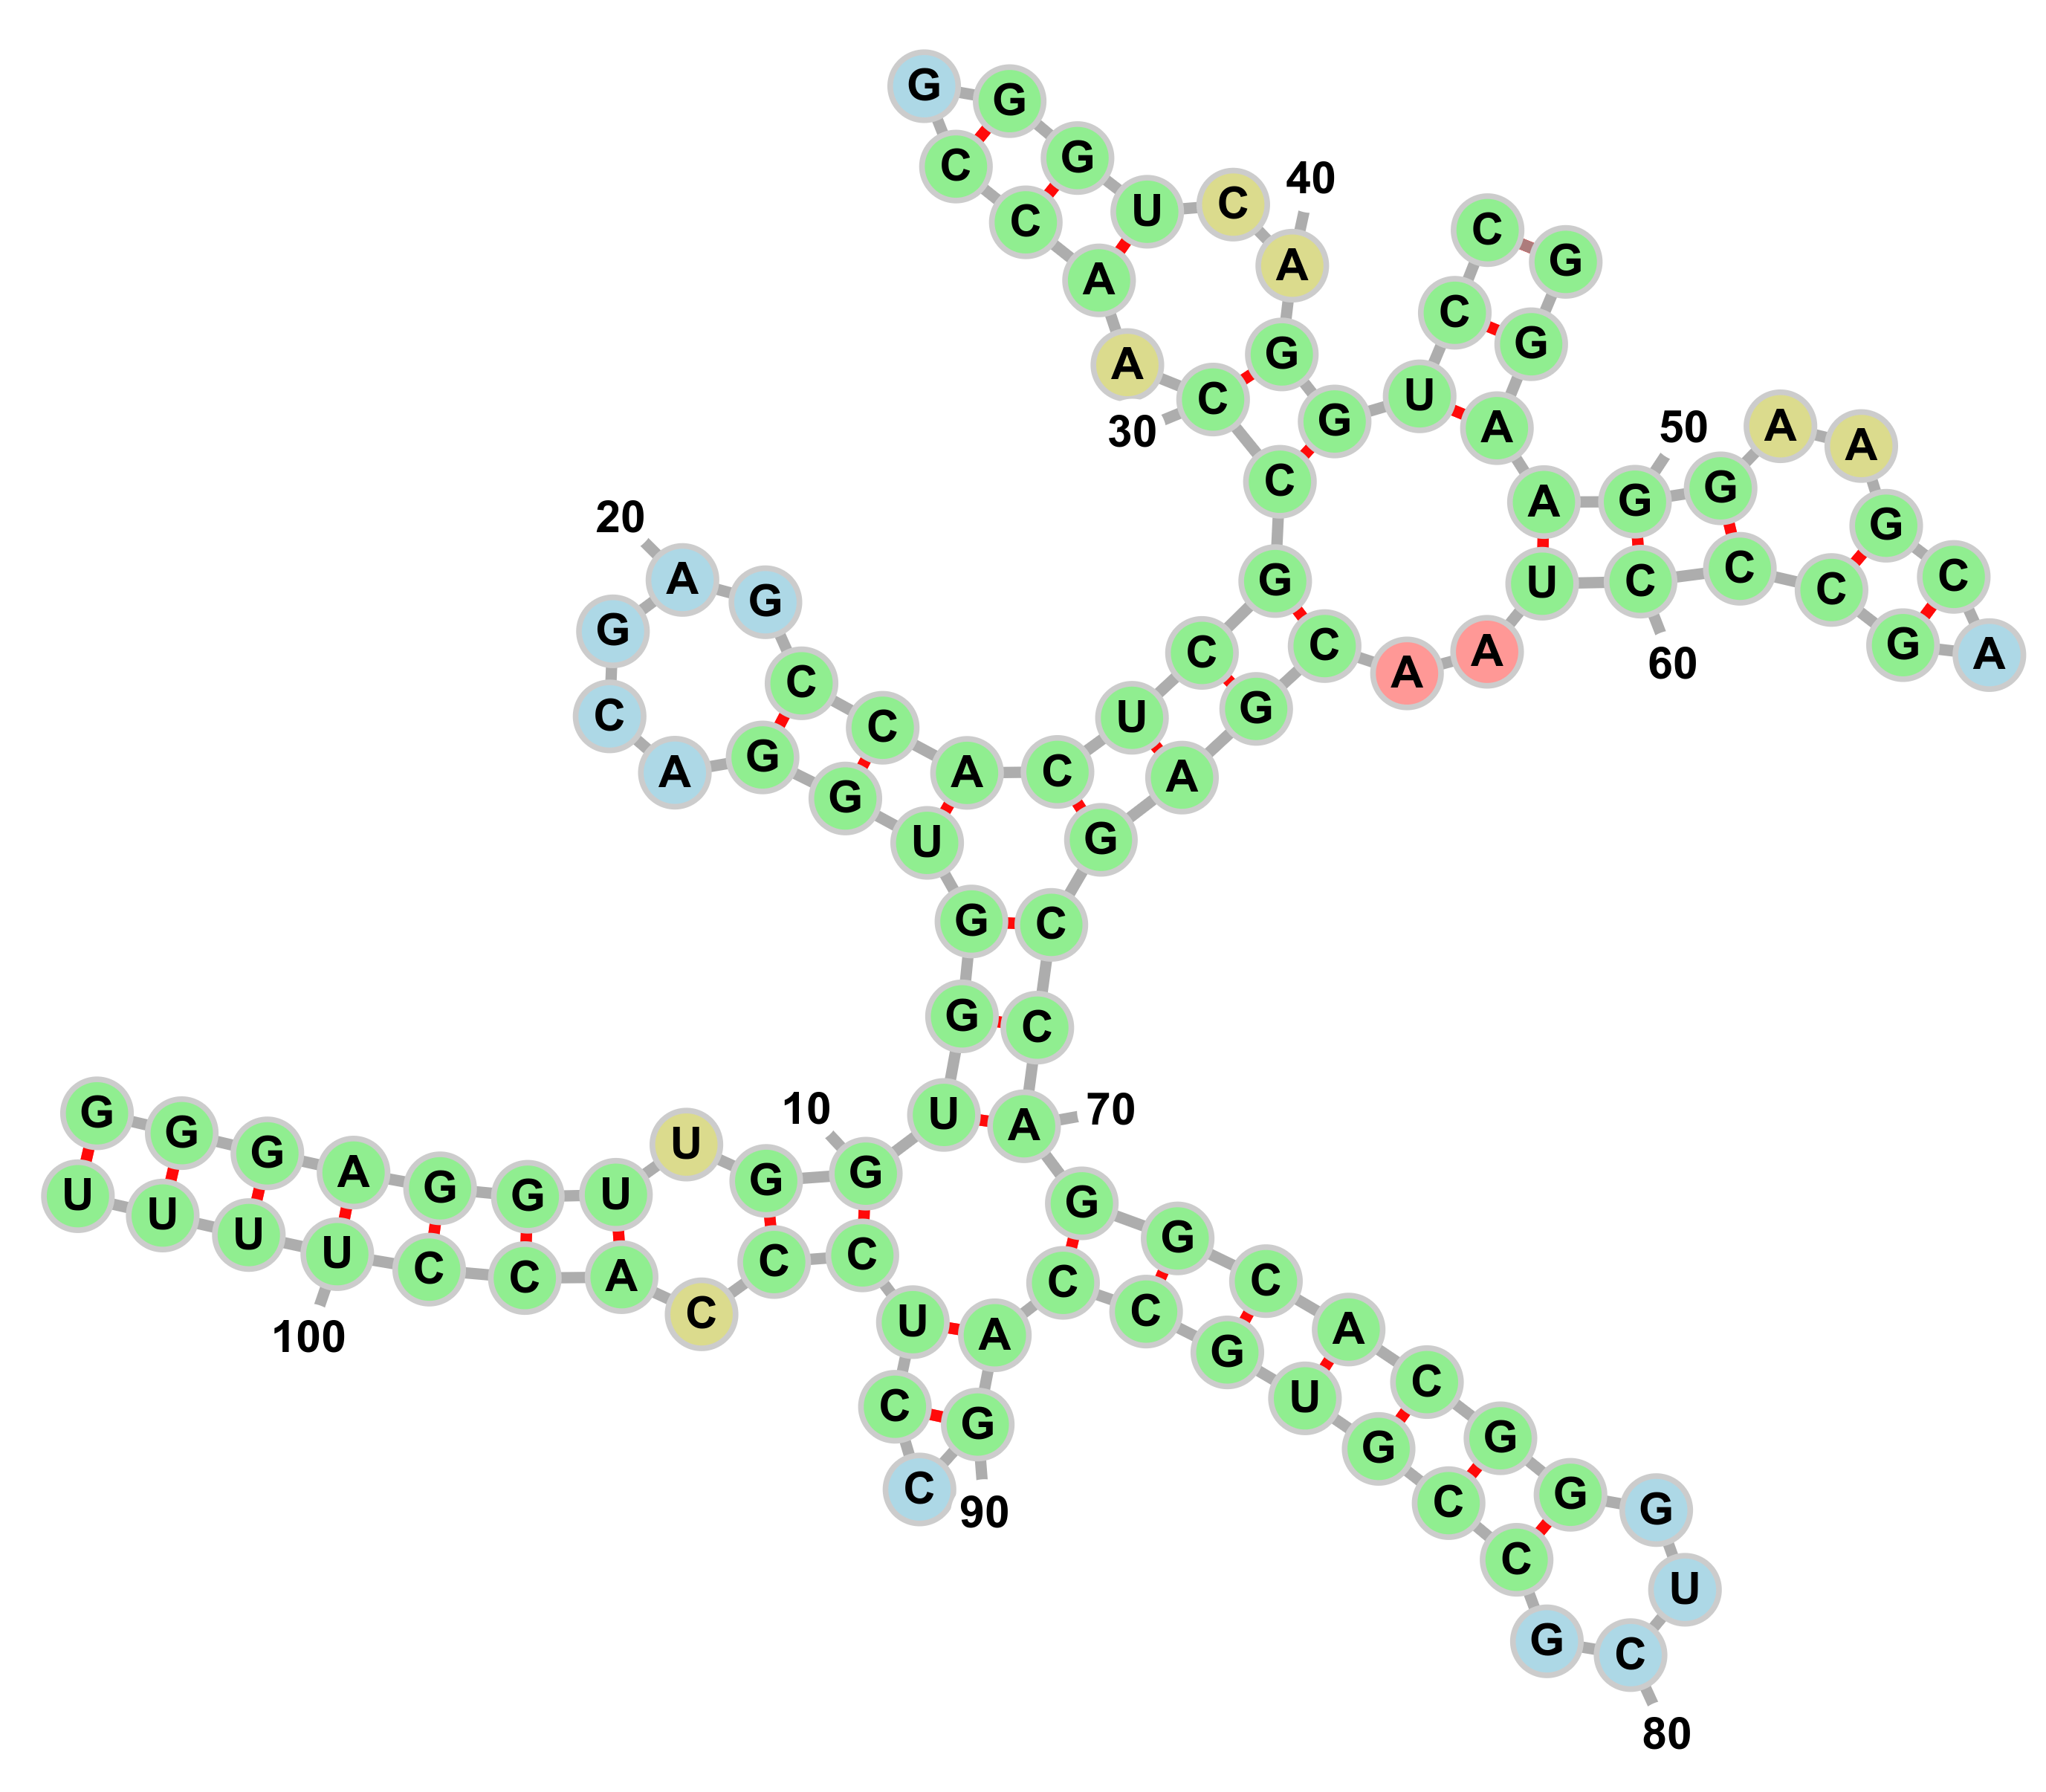
\includegraphics[width=\linewidth]{./img/SRP_00004_maxstacks.png}
        \caption{Maximize stacking pairs}
    \end{subfigure}
    \begin{subfigure}[b]{0.4\linewidth}
        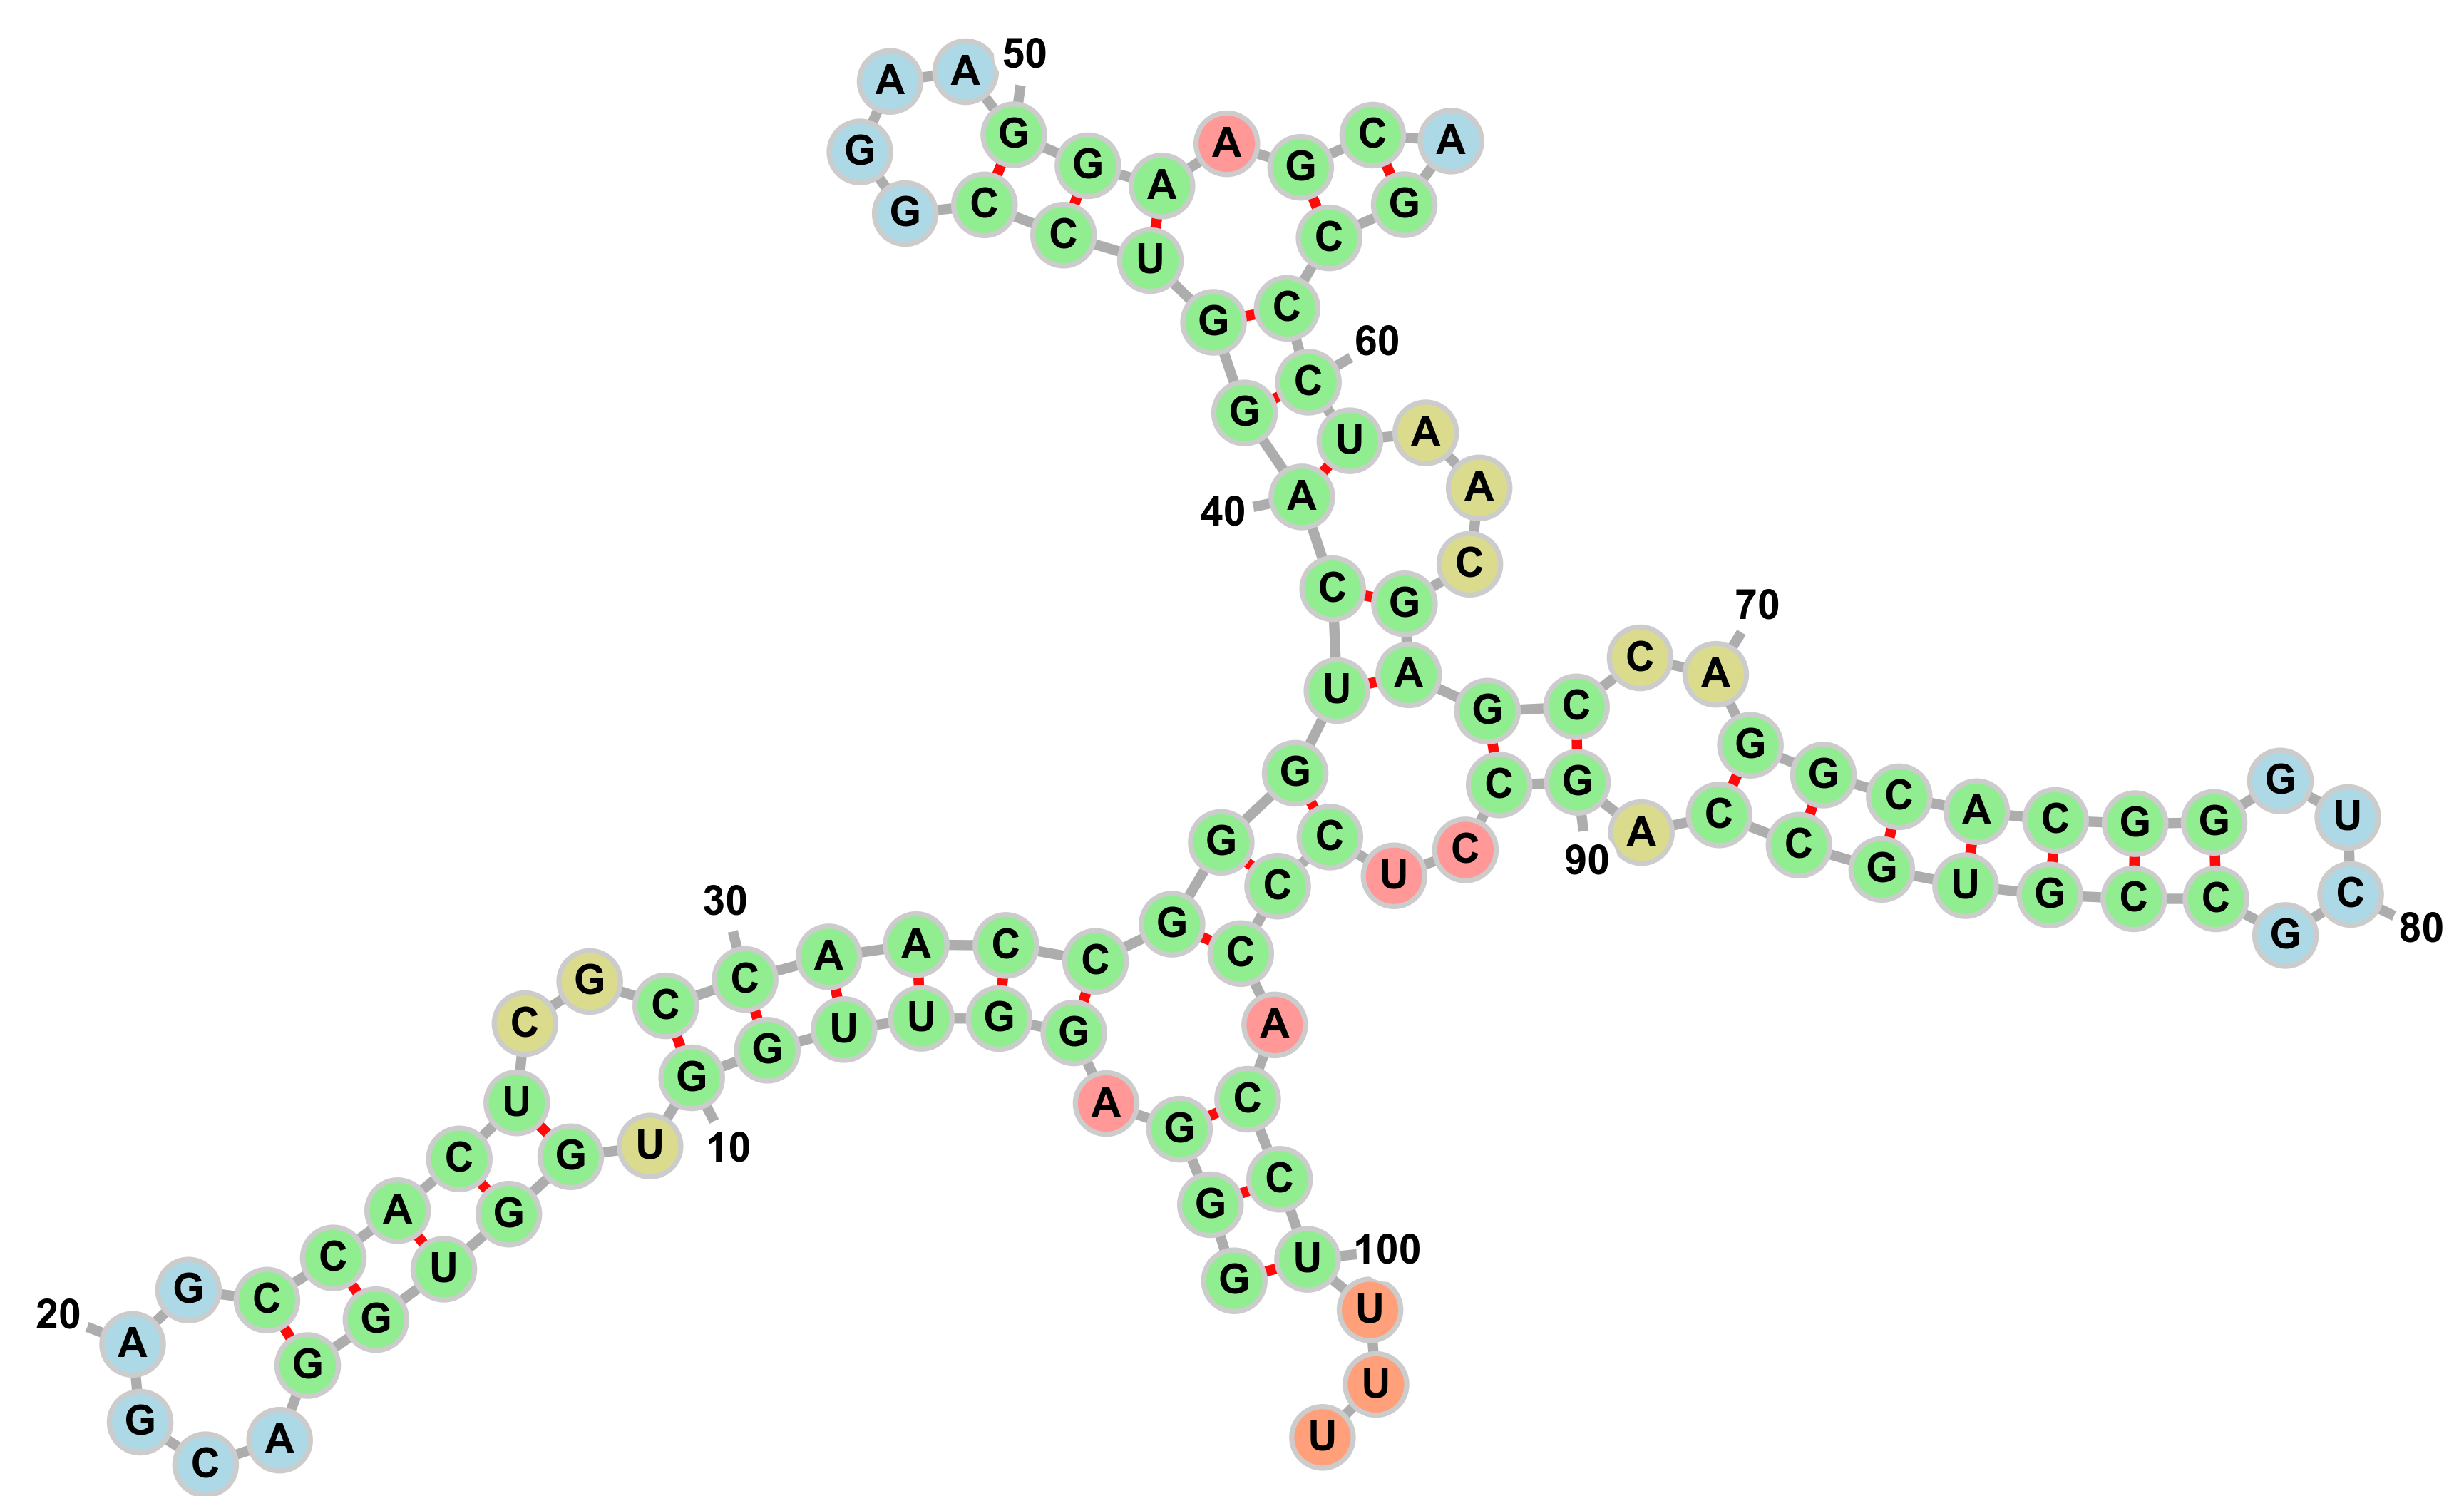
\includegraphics[width=\linewidth]{./img/SRP_00004_minstackenergy.png}
        \caption{Minimize stacking pairs energy}
    \end{subfigure}
    \begin{center}
        \begin{subfigure}[b]{\linewidth}
            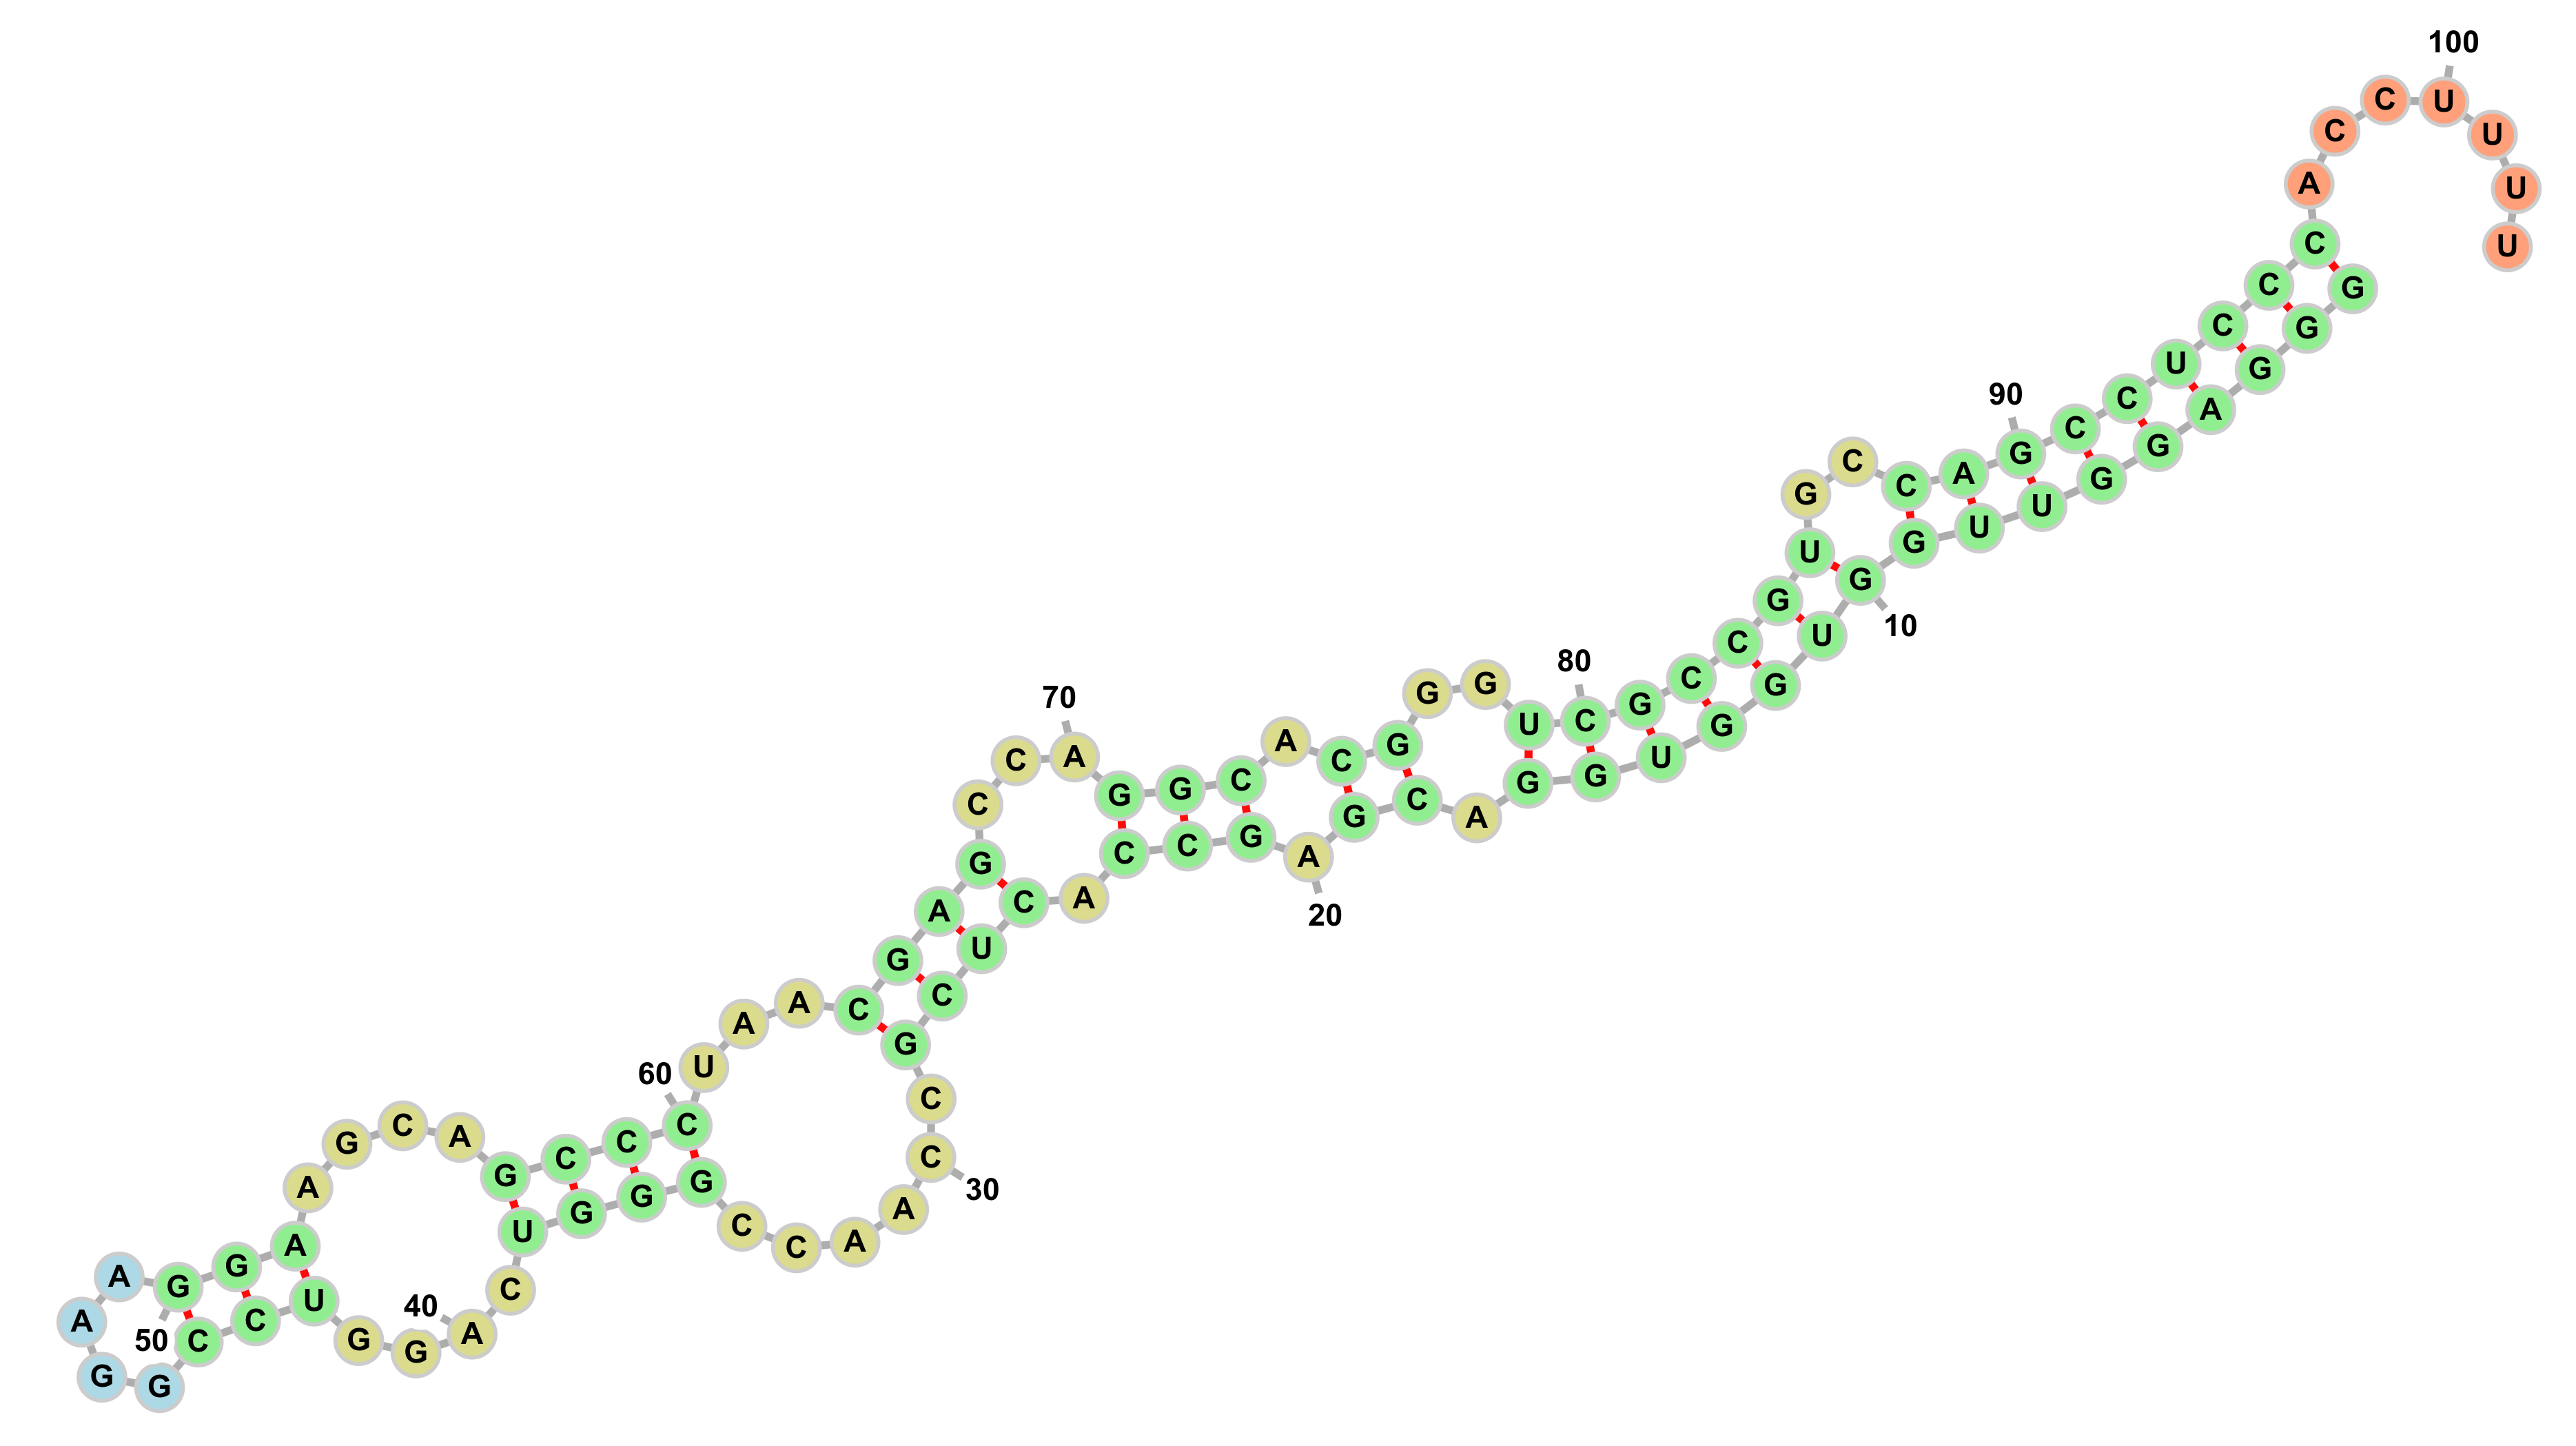
\includegraphics[width=\linewidth]{./img/SRP_00004_correct.png}
            \caption{Correct}
        \end{subfigure}
    \end{center}
\caption{SRP\_00004}
\label{fig:SRP_00004}
\end{figure}

\pagebreak

\subsection{Time consuming}
I tested the time consuming of each algorithm, result is shown in Fig.\ref{fig:time_consuming}.
From this result, we can see although these three algorithms has same time complexity, but the time consuming are
different. Nussinov is fastest, other two algorithms is similar.
This is because these two algoritms have an additional loop when fill the matrix and traceback compare to the Nussinov.

\begin{figure}[h]
    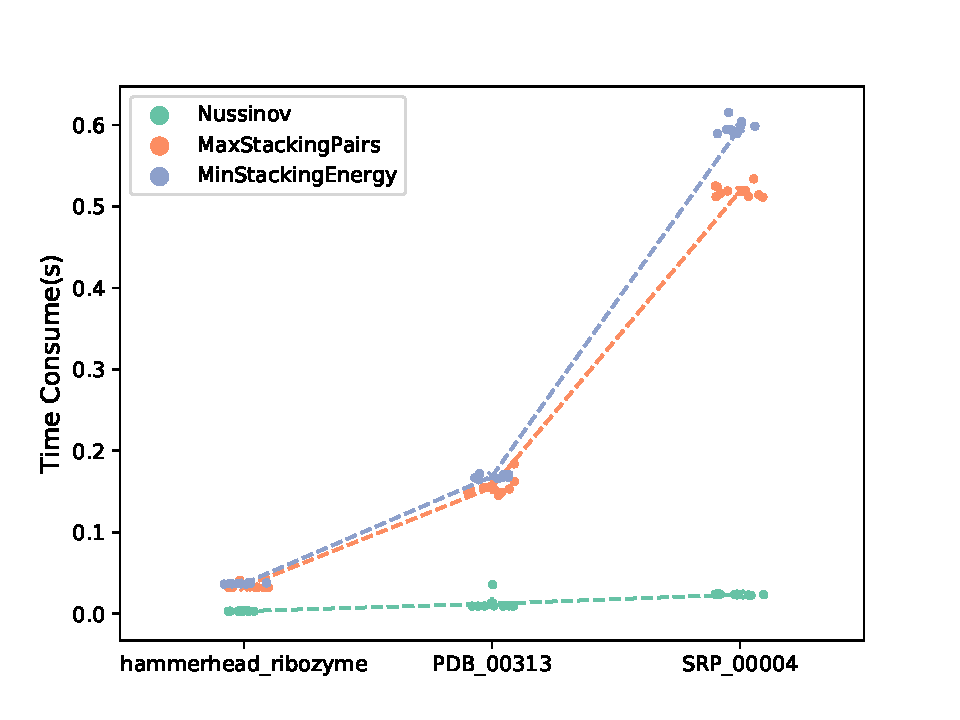
\includegraphics[width=\linewidth]{./img/time_consume.pdf}
    \caption{Time consuming of each algorithm}
    \label{fig:time_consuming}
\end{figure}

\section{Discussion}
\label{discussion}

From the results in the section \ref{sec:compare},
we can see that. 1. All these three algorithms can not predict the correct structure. I'm soo sorry.
2. Maximize stacking pairs and minimize stacking pairs energy methods produce the similar results.
3. Penalty for the short distance pairs can prohibit the formation of some incorrect short distance pairs.

The advantages of my score function is consider the real energy of each stacking pairs 
instead of just count the numbers. And I have considered the fact that, 
short distance pair is more unstable than long distance pairs, and this point indeed improved the results of prediction.
But my score function is not considered the energy of other secondary structures in addition to stacking pairs.
So it can not predict the structure correctly. And this method also can not predict the pseudo-knot structure.

At the same time, this implementation is also not good enough. At least two point can be improved: 
1. Python interpreter is not fast, if implement algorithm with C it will be much more faster.
2. Actually, in this implementation, the matrix for store scores only a half useful,
I can use hash table or sparse matrix to improve the memory usage.

\end{document}
